\documentclass[12pt, a4paper]{article}

% ============================================================================
% Paquetes
% ============================================================================
\usepackage[utf8]{inputenc}
% \usepackage[spanish]{babel}  % descomentar si texlive-lang-spanish está instalado
\usepackage{amsmath, amssymb}
\usepackage{graphicx}
\usepackage{float}
\usepackage{booktabs}
\usepackage{caption}
\usepackage{subcaption}
\usepackage[margin=2.5cm, headheight=15pt]{geometry}
\usepackage{hyperref}
\usepackage{fancyhdr}
\usepackage{listings}
\usepackage{xcolor}

% ============================================================================
% Configuración
% ============================================================================
\graphicspath{{figuras/}}

\hypersetup{
    colorlinks=true,
    linkcolor=blue,
    citecolor=blue,
    urlcolor=blue,
}

\pagestyle{fancy}
\fancyhf{}
\fancyhead[L]{TP1 — Sistemas de Control}
\fancyhead[R]{IOR442}
\fancyfoot[C]{\thepage}

\lstset{
    language=Python,
    basicstyle=\ttfamily\small,
    keywordstyle=\color{blue},
    commentstyle=\color{gray},
    stringstyle=\color{red},
    frame=single,
    breaklines=true,
}

% ============================================================================
\begin{document}

% --- Portada ---
\begin{titlepage}
\centering
\vspace*{2cm}
{\Large\textbf{Universidad Nacional de ...}}\\ % TODO: completar
\vspace{0.5cm}
{\large Facultad de ...}\\ % TODO: completar
\vspace{2cm}
{\LARGE\textbf{Trabajo Práctico N° 1}}\\\vspace{0.3cm}
{\Large Diseño de Controladores con Root Locus\\y Respuesta en Frecuencia}\\
\vspace{2cm}
{\large\textbf{Materia:} IOR442 — Sistemas de Control}\\
{\large\textbf{Profesor:} Dr. Mariano Scaramal}\\
\vspace{1.5cm}
{\large\textbf{Integrantes:}}\\
\vspace{0.3cm}
% TODO: completar con los nombres del grupo
Manuel Ramirez Silva - Legajo 34588\\
Agustin Federico Manzano - Legajo XXXXX\\
Maximo Simian Jacob - Legajo 34337\\
\vspace{2cm}
{\large Fecha de entrega: 22 de abril de 2026}

\vfill
\textbf{Entorno de desarrollo:}\\
Python 3.10 — NumPy 2.2.6 — SciPy 1.15.3 — Matplotlib 3.10.6 — python-control 0.10.2
\end{titlepage}

\tableofcontents
\newpage

% ============================================================================
% EJERCICIO 1
% ============================================================================
\section{Ejercicio 1: Sistema de Control de un Rotor de Aspas}

En este ejercicio se analiza un motor de corriente continua que acciona un rotor de aspas VTOL. El objetivo es diseñar un sistema de control capaz de seguir referencias de posición angular y rechazar perturbaciones de carga.

\subsection{Modelo del sistema}

La dinámica del motor DC se rige por tres ecuaciones diferenciales:

\begin{align}
    L\frac{di}{dt} + Ri + K_e\omega &= V(t) \label{eq:electrica}\\
    J\frac{d\omega}{dt} + B\omega &= K_t i(t) \label{eq:mecanica}\\
    \omega &= \frac{d\theta}{dt} \label{eq:cinematica}
\end{align}

\noindent con los parámetros de la Tabla~\ref{tab:parametros}.

\begin{table}[H]
\centering
\caption{Parámetros del motor DC.}
\label{tab:parametros}
\begin{tabular}{@{}clcl@{}}
\toprule
\textbf{Símbolo} & \textbf{Descripción} & \textbf{Valor} & \textbf{Unidad} \\
\midrule
$L$   & Inductancia de armadura       & 0,15  & H \\
$R$   & Resistencia de armadura       & 0,7   & $\Omega$ \\
$K_e$ & Constante de FEM              & 0,1   & V$\cdot$s/rad \\
$J$   & Momento de inercia total      & 0,02  & kg$\cdot$m$^2$ \\
$B$   & Coeficiente de fricción viscosa & 0,25 & N$\cdot$m$\cdot$s/rad \\
$K_t$ & Constante de torque           & 0,25  & N$\cdot$m/A \\
\bottomrule
\end{tabular}
\end{table}

% -------------------------------------------------------------------------
\subsection{Parte A — Análisis del Sistema}
% -------------------------------------------------------------------------

\subsubsection{A.a) Función de transferencia y variables de estado}

Aplicando la transformada de Laplace a las ecuaciones (\ref{eq:electrica})--(\ref{eq:cinematica}) con condiciones iniciales nulas, se obtiene:
%
\begin{equation}
    G(s) = \frac{\Theta(s)}{V(s)} = \frac{K_t}{s\left[(Ls+R)(Js+B) + K_eK_t\right]}
\end{equation}

Expandiendo el denominador con los valores numéricos:
%
\begin{equation}
    G(s) = \frac{0{,}25}{s\,(0{,}003\,s^2 + 0{,}0515\,s + 0{,}2)}
    = \frac{83{,}33}{s\,(s^2 + 17{,}17\,s + 66{,}67)}
    \label{eq:Gs}
\end{equation}

El sistema es de \textbf{Tipo 1} (un integrador puro), con tres polos reales:
%
\begin{equation}
    s_1 = 0, \quad s_2 \approx -5{,}94, \quad s_3 \approx -11{,}23
\end{equation}

\noindent El discriminante del polinomio cuadrático es $\Delta = 0{,}0515^2 - 4 \cdot 0{,}003 \cdot 0{,}2 = 2{,}52 \times 10^{-4} > 0$, confirmando que los polos son reales y no complejos conjugados. El polo dominante (excluyendo el integrador) es $s_2 \approx -5{,}94$.

\paragraph{Variables de estado.} Eligiendo $\mathbf{x} = [\theta,\; \omega,\; i]^T$:
%
\begin{equation}
\dot{\mathbf{x}} =
\begin{bmatrix} 0 & 1 & 0 \\ 0 & -12{,}5 & 12{,}5 \\ 0 & -0{,}667 & -4{,}667 \end{bmatrix} \mathbf{x}
+ \begin{bmatrix} 0 \\ 0 \\ 6{,}667 \end{bmatrix} V, \quad
y = \begin{bmatrix} 1 & 0 & 0 \end{bmatrix} \mathbf{x}
\end{equation}

Se verificó numéricamente que la conversión de espacio de estados a función de transferencia reproduce la ecuación (\ref{eq:Gs}).

% --- A.b ---
\subsubsection{A.b) Márgenes de ganancia y fase}

La Figura~\ref{fig:bode_planta} muestra el diagrama de Bode de $G(s)$ a lazo abierto.

\begin{figure}[H]
\centering
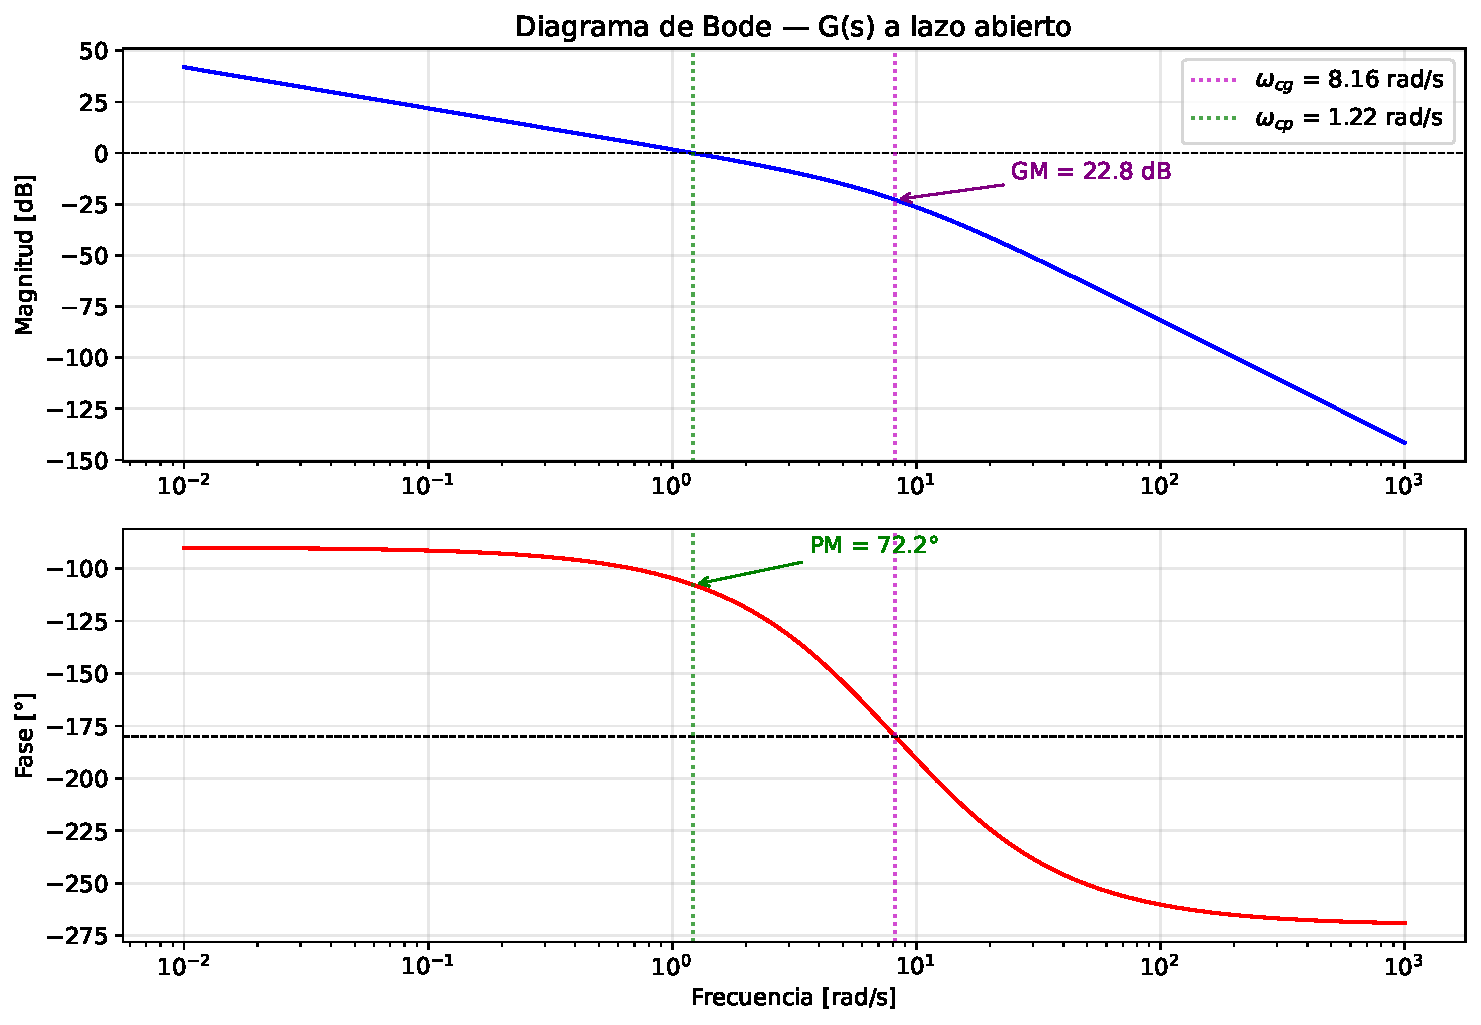
\includegraphics[width=0.85\textwidth]{bode_planta.pdf}
\caption{Diagrama de Bode de $G(s)$ con indicación de márgenes de estabilidad.}
\label{fig:bode_planta}
\end{figure}

Los márgenes obtenidos son:
%
\begin{table}[H]
\centering
\caption{Márgenes de estabilidad del sistema sin compensar.}
\begin{tabular}{@{}lcc@{}}
\toprule
\textbf{Parámetro} & \textbf{Valor} & \textbf{Frecuencia} \\
\midrule
Margen de ganancia (GM) & 22,8 dB & $\omega_{cg} = 8{,}16$ rad/s \\
Margen de fase (PM)     & 72,2°   & $\omega_{cp} = 1{,}22$ rad/s \\
\bottomrule
\end{tabular}
\end{table}

Ambos márgenes son positivos y amplios (GM $>$ 6\,dB, PM $>$ 45°), lo cual indica que el sistema en lazo cerrado con $C(s)=1$ es estable y tiene buena robustez de estabilidad. El sistema sin compensar ya satisface los criterios de transitorio ($t_s$ y $M_p$); sin embargo, como se demostrará en la Parte~B, la especificación de \textbf{rechazo de perturbación} (error $< 5\,\%$ ante torque de carga del 20\,\% de la referencia) \textbf{no se cumple} ($e_{pert} \approx 64\,\%$), lo que motiva el diseño de un controlador.

% --- A.c ---
\subsubsection{A.c) Respuesta ante escalón con perturbación de carga}

La perturbación de torque $n(t)$ entra en la ecuación mecánica. La transferencia $\Theta(s)/N(s)$ se obtiene anulando la referencia ($R = 0$) y reduciendo el diagrama de bloques. Con $E(s) = -\Theta(s)$ (error de realimentación) y $G_n(s) = 1/[s(Js+B)]$ la transferencia en lazo abierto de perturbación a ángulo:
%
\begin{align}
    \Theta(s) &= G(s)\,E(s) + G_n(s)\,N(s) = -G(s)\,\Theta(s) + G_n(s)\,N(s) \nonumber\\
    \Theta(s)\,[1 + G(s)] &= G_n(s)\,N(s) \nonumber\\
    \frac{\Theta(s)}{N(s)} &= \frac{G_n(s)}{1+G(s)} \label{eq:Tpert}
\end{align}

Por superposición con referencia no nula:
%
\begin{equation}
    \Theta(s) = \underbrace{\frac{G(s)}{1+G(s)}}_{T_{ref}(s)} R(s)
    + \underbrace{\frac{G_n(s)}{1+G(s)}}_{T_{pert}(s)} N(s)
\end{equation}

La Figura~\ref{fig:escalon_pert} muestra la respuesta del sistema ante un escalón unitario y una perturbación de carga de magnitud 0,1 aplicadas simultáneamente.

\begin{figure}[H]
\centering
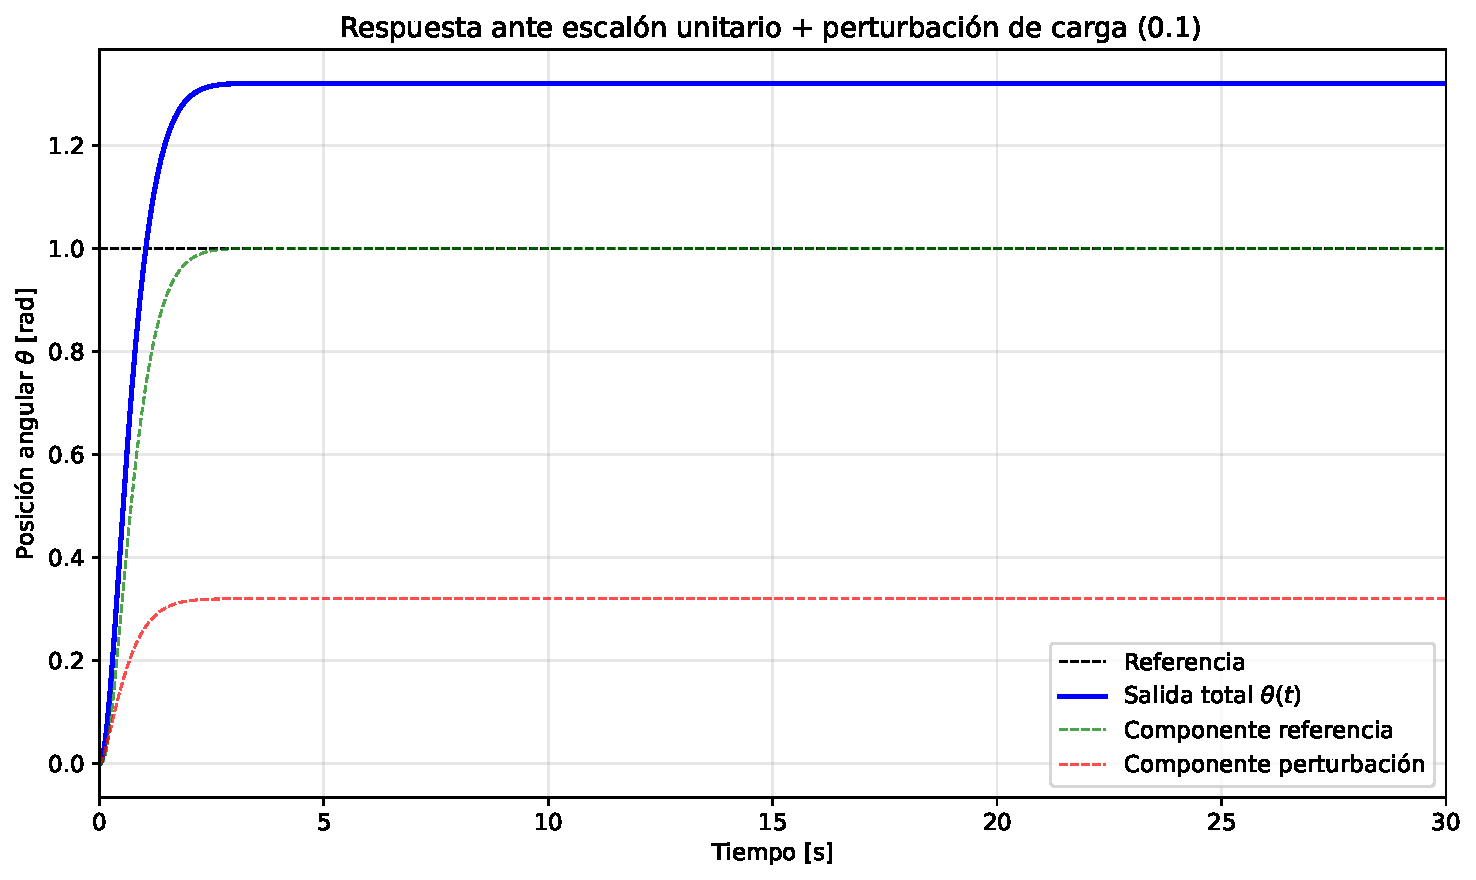
\includegraphics[width=0.85\textwidth]{escalon_perturbacion.pdf}
\caption{Respuesta ante escalón unitario + perturbación de carga (0,1). Se muestra la salida total y las componentes individuales por superposición.}
\label{fig:escalon_pert}
\end{figure}

Al ser Tipo~1, la referencia escalón se sigue con \textbf{error nulo} ($K_p = \infty$). Sin embargo, la perturbación constante produce un \textbf{offset en régimen permanente significativo}: el error estacionario es $\theta_{pert,\infty} = G_n(0)/[1{+}G(0)] \cdot N_0$, que para $C(s)=1$ resulta en $3{,}2 \times N_0$~rad. Con la perturbación de amplitud 0,1 del ejemplo, esto implica un desvío de 0,32~rad (32\,\%). Para eliminar este error se requiere un integrador en el controlador (Tipo~2).

% --- A.d ---
\subsubsection{A.d) Respuesta ante rampa con perturbación de carga}

Para una referencia rampa $r(t) = t$, el error en régimen permanente depende de la constante de velocidad:
%
\begin{equation}
    e_{ss} = \frac{1}{K_v}, \quad K_v = \lim_{s \to 0} s \cdot G(s)
\end{equation}

Al ser Tipo~1, $K_v$ es finito, por lo que el sistema \textbf{no puede seguir la rampa con error nulo}.

\begin{figure}[H]
\centering
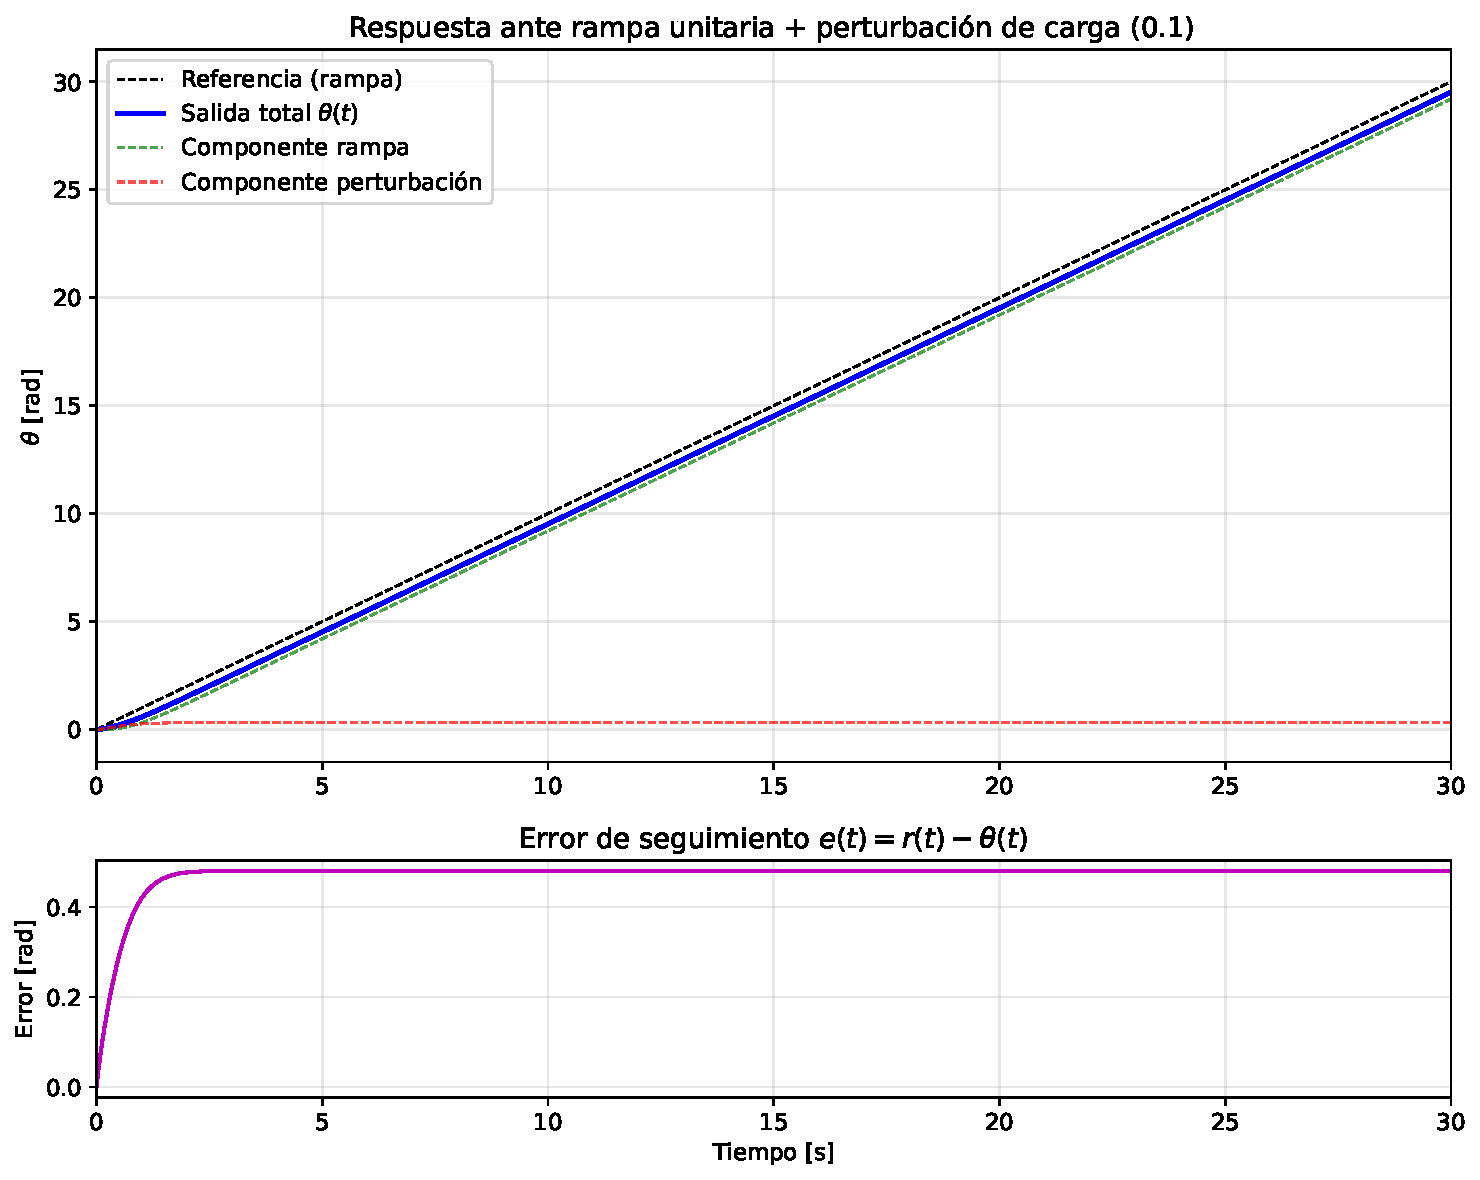
\includegraphics[width=0.85\textwidth]{rampa_perturbacion.pdf}
\caption{Respuesta ante rampa unitaria + perturbación de carga (0,1). El error de seguimiento converge a un valor constante $1/K_v$.}
\label{fig:rampa_pert}
\end{figure}

% --- A.e ---
\subsubsection{A.e) Propuesta de controlador}

\begin{table}[H]
\centering
\caption{Propuesta de controladores según el escenario.}
\begin{tabular}{@{}p{3.5cm}p{3.5cm}p{6cm}@{}}
\toprule
\textbf{Escenario} & \textbf{Controlador} & \textbf{Justificación} \\
\midrule
Escalón + perturbación & Lead (adelanto) & Aporta fase positiva, mejora $t_s$ y $M_p$. Mayor ganancia a frecuencias medias mejora rechazo de perturbación. \\
\addlinespace
Rampa + perturbación & Lead + Integrador & El integrador aumenta el tipo a 2 ($K_v=\infty$). El lead compensa la pérdida de margen de fase. \\
\bottomrule
\end{tabular}
\end{table}

\noindent\textbf{¿Por qué no un compensador lag?} Un lag mejoraría la precisión en baja frecuencia pero reduciría el ancho de banda, empeorando el transitorio. Como las especificaciones exigen buen transitorio \emph{y} precisión, se prefiere lead para el primer caso y lead+integrador para el segundo.

% -------------------------------------------------------------------------
\subsection{Parte B — Diseño del Sistema de Control}
% -------------------------------------------------------------------------

\subsubsection{B.a) Evaluación del sistema sin compensar}

Las especificaciones de desempeño ante escalón unitario son:

\begin{table}[H]
\centering
\caption{Especificaciones de diseño.}
\begin{tabular}{@{}lcc@{}}
\toprule
\textbf{Requisito} & \textbf{Valor} & \textbf{Restricción en plano $s$} \\
\midrule
$t_s \leq 7{,}5$ s (2\%) & $\sigma \geq 0{,}533$ rad/s & $\text{Re}(s) \leq -0{,}533$ \\
$M_p \leq 15\%$          & $\zeta \geq 0{,}517$        & Cono de amortiguamiento \\
Error pert. $< 5\%$ (pert. 20\%) & --- & Ganancia suficiente \\
\bottomrule
\end{tabular}
\end{table}

La Figura~\ref{fig:escalon_sin} muestra la respuesta del sistema sin compensar ($C(s)=1$) ante escalón unitario.

\begin{figure}[H]
\centering
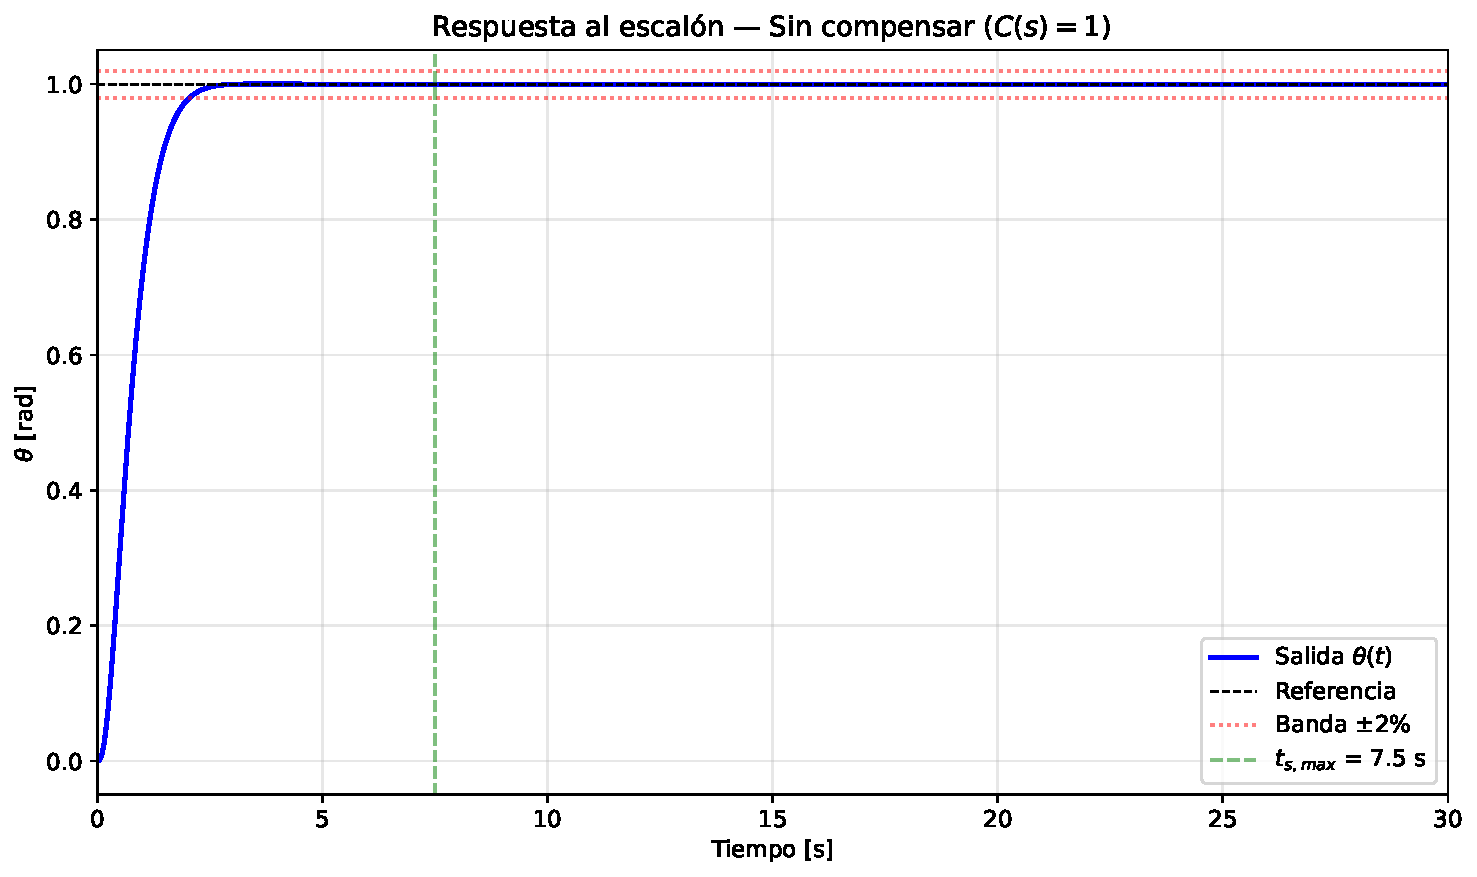
\includegraphics[width=0.85\textwidth]{escalon_sin_compensar.pdf}
\caption{Respuesta al escalón del sistema sin compensar, con banda del 2\% y $t_{s,max}$.}
\label{fig:escalon_sin}
\end{figure}

\begin{table}[H]
\centering
\caption{Evaluación del sistema \textbf{sin compensar} ($C(s)=1$) ante escalón unitario + perturbación 20\,\%.}
\begin{tabular}{@{}lccl@{}}
\toprule
\textbf{Requisito} & \textbf{Obtenido} & \textbf{Límite} & \textbf{Cumple} \\
\midrule
$t_s$ & 2,05~s  & $\leq 7{,}5$~s & \checkmark \\
$M_p$ & 0,0\,\% & $\leq 15\,\%$  & \checkmark \\
$e_{pert}$ & 64,0\,\% & $< 5\,\%$ & $\times$ \\
\bottomrule
\end{tabular}
\end{table}

El sistema sin compensar ya satisface los criterios de transitorio ($t_s$, $M_p$), pero falla en el rechazo de perturbación: la respuesta estacionaria ante el torque de carga se desvía un 64\,\% de la referencia. Este es el motivo que justifica el diseño de un controlador.

\subsubsection{B.b) Diseño del controlador por Root Locus}

\paragraph{Polo dominante deseado.} Se elige con margen sobre las restricciones mínimas:
%
\begin{equation}
    \sigma_d = 0{,}7 \;\text{rad/s}, \quad \zeta_d = 0{,}6 \quad \Rightarrow \quad
    s_d = -0{,}7 + j\,0{,}933
\end{equation}

\paragraph{Contribución angular.} Se evalúa $\angle G(s_d)$ y se calcula la fase que debe aportar el compensador lead para que $s_d$ pertenezca al root locus:
%
\begin{equation}
    \angle C(s_d) = -180^{\circ} - \angle G(s_d)
\end{equation}

\paragraph{Ubicación del cero y polo.} Se coloca el cero en $z_c = -2$ (entre el origen y el polo dominante de la planta en $-5{,}94$) para atraer el root locus hacia la región admisible. El polo $p_c$ se calcula para satisfacer la contribución angular requerida.

\paragraph{Ajuste de ganancia.} Se aplica la condición de magnitud:
%
\begin{equation}
    K_c = \frac{1}{|C(s_d) \cdot G(s_d)|}
\end{equation}

El compensador resultante es:
%
\begin{equation}
    C(s) = 0{,}4785 \cdot \frac{s + 2{,}0000}{s + 0{,}9741}
\end{equation}

La Figura~\ref{fig:rlocus_sin} muestra el root locus del sistema sin compensar con la región admisible sombreada, y la Figura~\ref{fig:rlocus_comp} el root locus del sistema compensado con los polos de lazo cerrado marcados.

\begin{figure}[H]
\centering
\begin{subfigure}[t]{0.48\textwidth}
    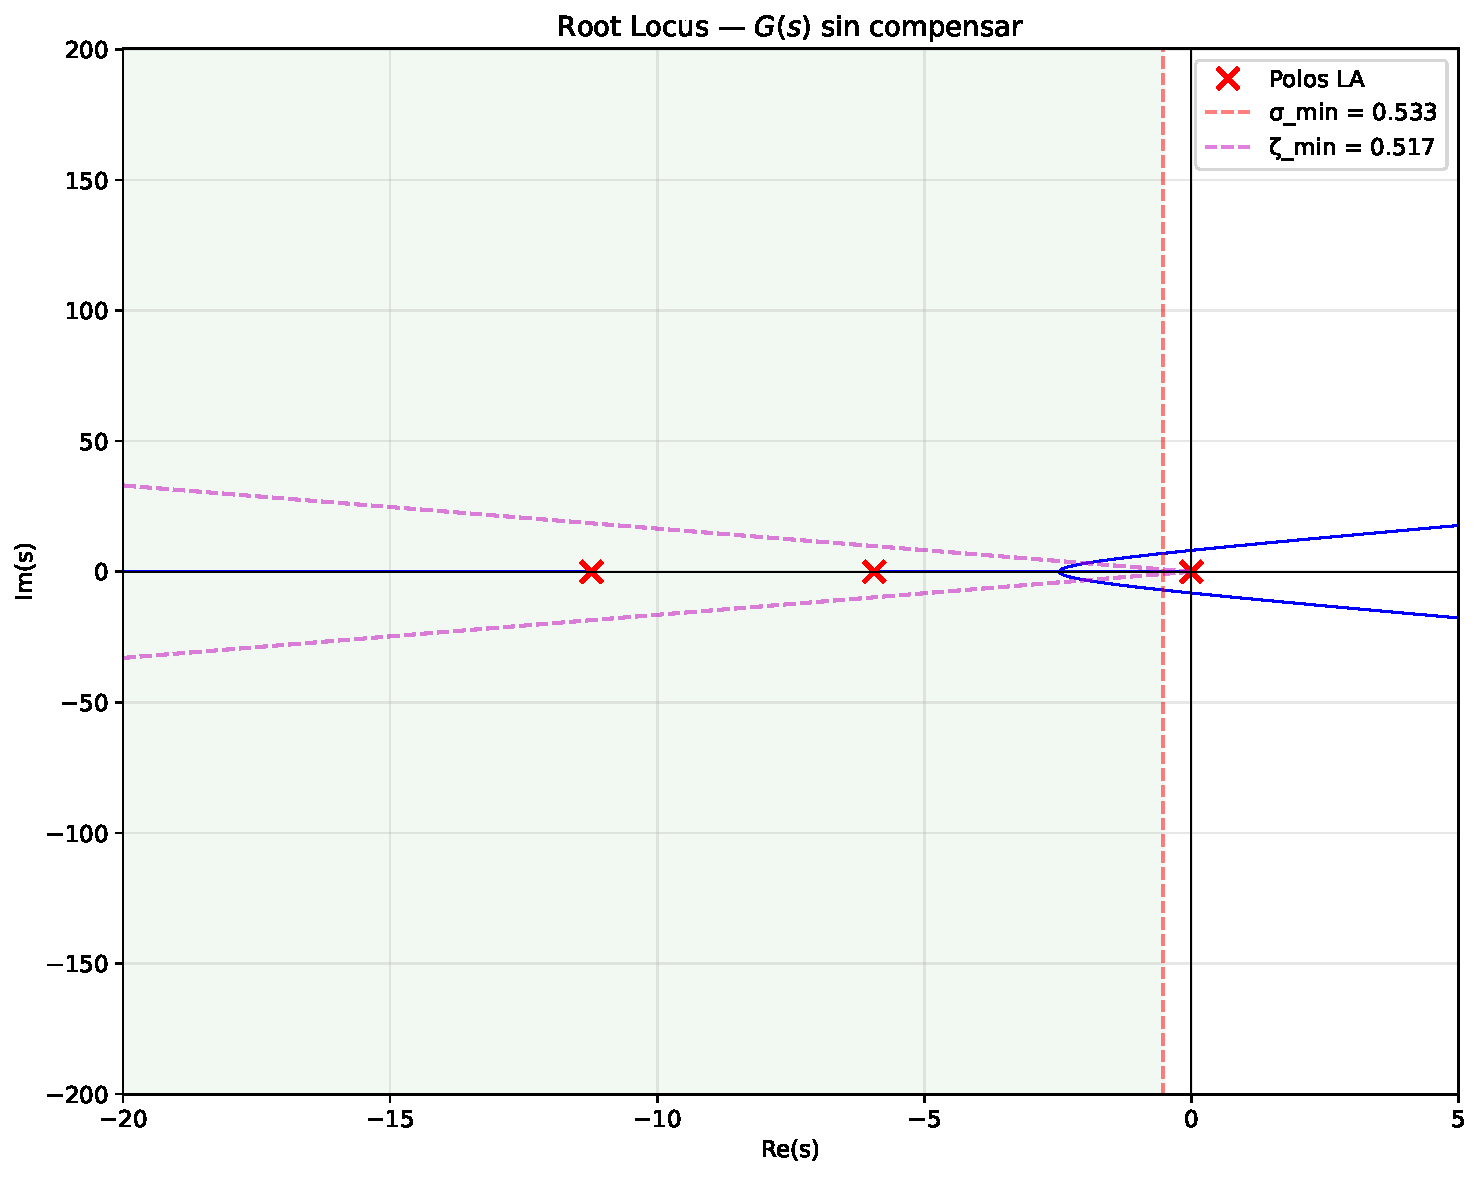
\includegraphics[width=\textwidth]{rlocus_sin_compensar.pdf}
    \caption{Sin compensar.}
    \label{fig:rlocus_sin}
\end{subfigure}
\hfill
\begin{subfigure}[t]{0.48\textwidth}
    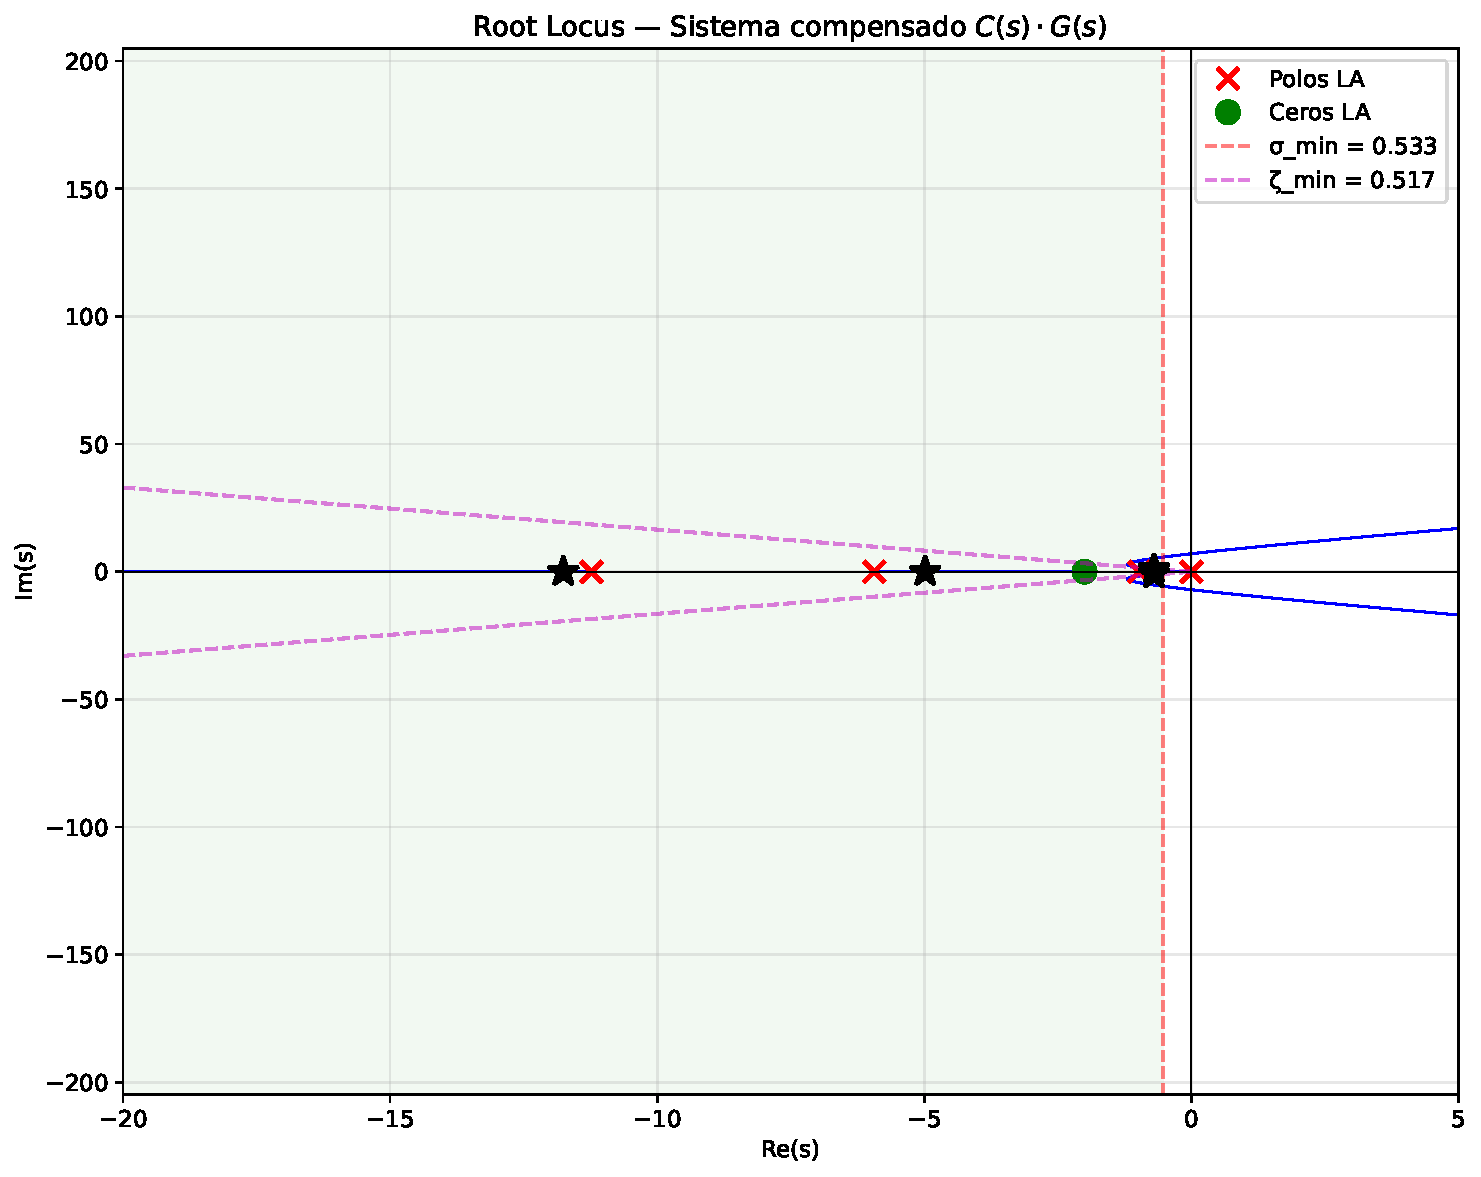
\includegraphics[width=\textwidth]{rlocus_compensado.pdf}
    \caption{Compensado (estrellas = polos LC).}
    \label{fig:rlocus_comp}
\end{subfigure}
\caption{Root Locus con región admisible ($\sigma_{min}$, $\zeta_{min}$).}
\end{figure}

La Figura~\ref{fig:escalon_comp} compara la respuesta al escalón con perturbación del 20\% para ambos sistemas.

\begin{figure}[H]
\centering
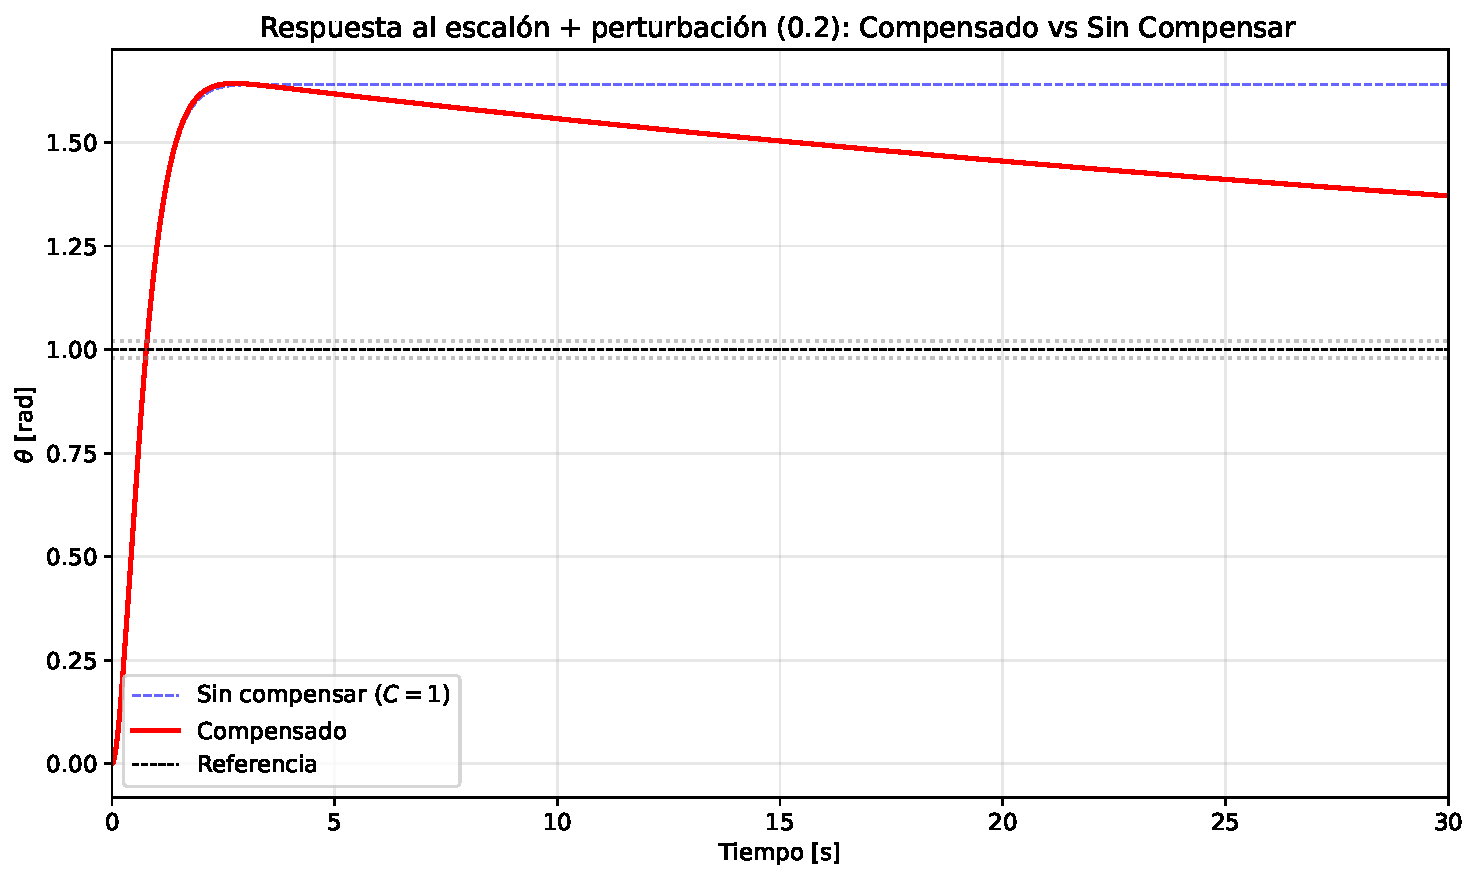
\includegraphics[width=0.85\textwidth]{escalon_comp_vs_sin.pdf}
\caption{Respuesta al escalón + perturbación (0,2): compensado vs sin compensar.}
\label{fig:escalon_comp}
\end{figure}

\begin{table}[H]
\centering
\caption{Evaluación del sistema \textbf{compensado} ante escalón unitario + perturbación 20\,\%.}
\begin{tabular}{@{}lccl@{}}
\toprule
\textbf{Requisito} & \textbf{Obtenido} & \textbf{Límite} & \textbf{Cumple} \\
\midrule
$t_s$ & 4,84~s   & $\leq 7{,}5$~s & \checkmark \\
$M_p$ & 11,65\,\% & $\leq 15\,\%$ & \checkmark \\
$e_{pert}$ & 65,1\,\% & $< 5\,\%$ & $\times$ \\
\bottomrule
\end{tabular}
\end{table}

El compensador lead mejora el transitorio ($t_s$, $M_p$) pero \textbf{no resuelve el rechazo de perturbación}: el error estacionario ante torque de carga se mantiene en $\approx 65\,\%$, ya que la ganancia DC del compensador es $C(0) = 0{,}9742 \approx 1$.

\paragraph{¿Por qué el lead no puede cumplir la especificación de perturbación?} Para un sistema Tipo~1, el error en régimen permanente ante perturbación constante $N_0$ es:
%
\begin{equation}
    e_{pert,\infty} = \frac{G_n(0)/G(0)}{C(0)} \cdot N_0 = \frac{3{,}2}{C(0)} \cdot N_0
\end{equation}
%
Con $C(0)\approx 1$ se obtiene $e_{pert}=64\,\%$ para $N_0=0{,}2$. Para cumplir $e_{pert} < 5\,\%$ se necesitaría $C(0) > 12{,}8$, es decir, una ganancia DC de lazo al menos 12,8 veces mayor. Un compensador lead \emph{normalizado} con $C(0)=1$ no modifica esta ganancia y, por tanto, no puede reducir el error. Las alternativas son:
\begin{itemize}
    \item \textbf{Controlador proporcional de alta ganancia} ($K > 12{,}8$): aumenta el DC de lazo pero incrementa el ancho de banda y puede violar $M_p \leq 15\,\%$.
    \item \textbf{Integrador} (Tipo~2): hace $e_{pert} = 0$, pero reduce el margen de fase y típicamente aumenta el sobrepico (véase Parte~B.e).
\end{itemize}
La especificación de rechazo de perturbación no puede cumplirse simultáneamente con las de transitorio mediante un lead simple; se requeriría un controlador de mayor complejidad (PID o lead-lag con integrador).

\subsubsection{B.c) Márgenes de ganancia y fase — Comparación Bode}

\begin{figure}[H]
\centering
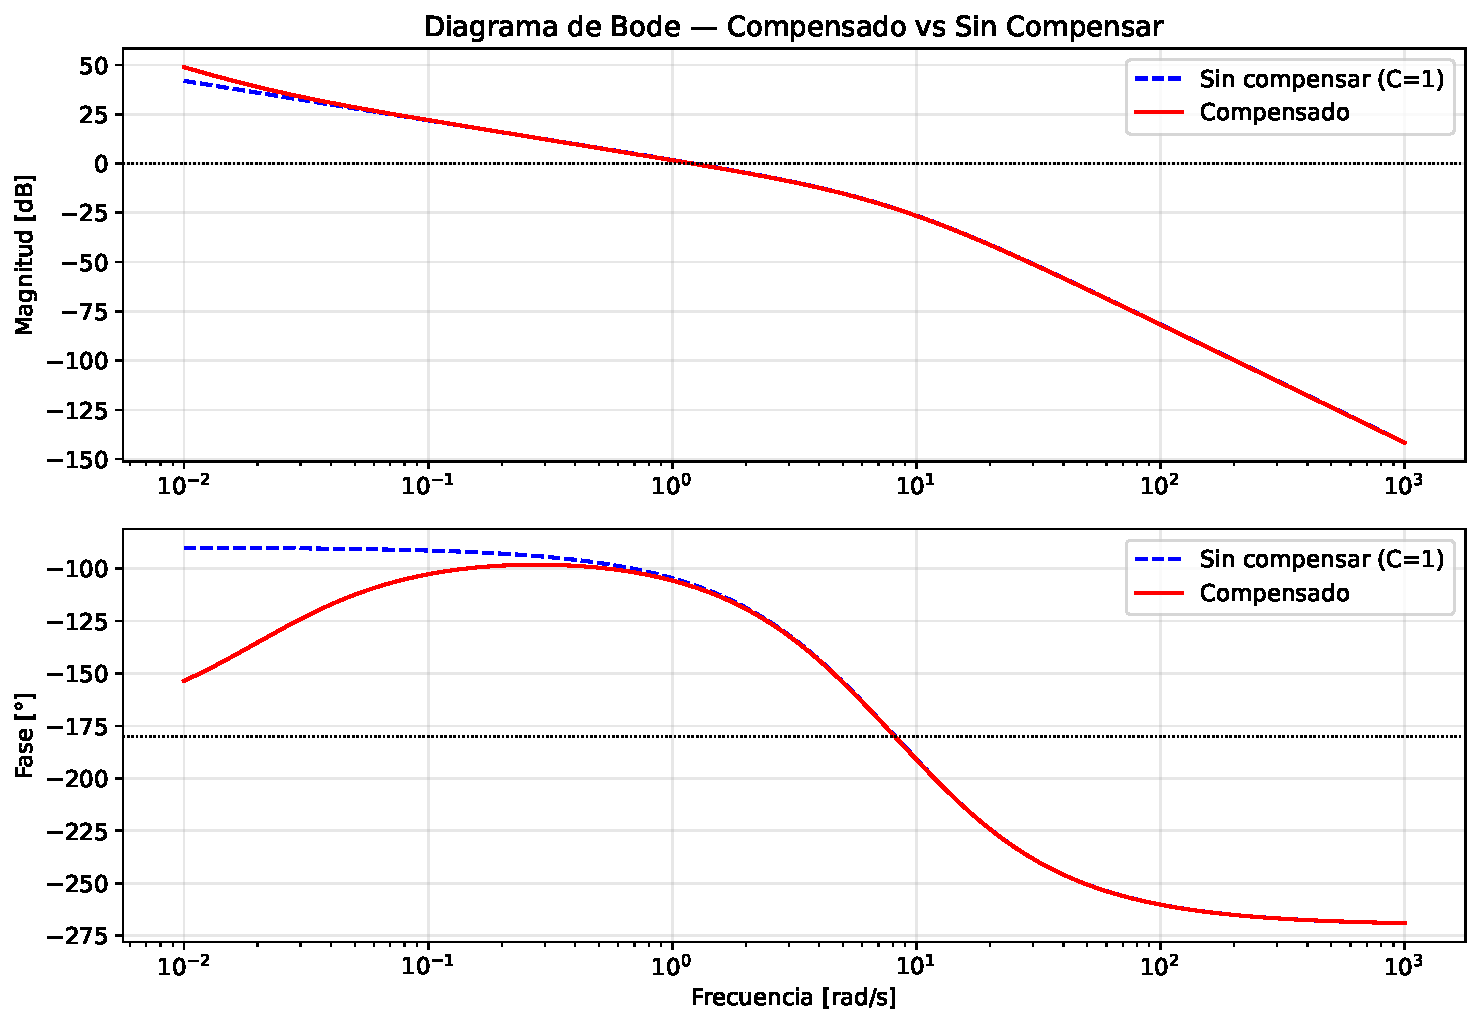
\includegraphics[width=0.85\textwidth]{bode_comparativo.pdf}
\caption{Diagrama de Bode: sistema compensado vs sin compensar.}
\label{fig:bode_comp}
\end{figure}

\begin{table}[H]
\centering
\caption{Comparación de márgenes de estabilidad.}
\begin{tabular}{@{}lccc@{}}
\toprule
& \textbf{Sin compensar} & \textbf{Compensado} \\
\midrule
GM [dB]         & 22,8   & 26,4 \\
PM [°]          & 72,2   & 57,1 \\
$\omega_{cg}$ [rad/s] & 8,16 & 7,05 \\
$\omega_{cp}$ [rad/s] & 1,22 & 0,96 \\
\bottomrule
\end{tabular}
\end{table}

El compensador lead reduce el PM de 72,2° a 57,1°, porque aportó fase positiva en la banda media pero desplazó la frecuencia de cruce $\omega_{cp}$ hacia un valor menor (1,22 → 0,96~rad/s), región donde la planta tiene mayor atraso de fase. Al mismo tiempo, el GM aumentó de 22,8~dB a 26,4~dB: el compensador alejó la ganancia de cruce de la frecuencia de ganancia unitaria, otorgando mayor margen antes de llegar a la inestabilidad por ganancia. En resumen, el lead mejoró la robustez de ganancia a costa de reducir el margen de fase.

\subsubsection{B.d) Seguimiento de rampa}

\begin{figure}[H]
\centering
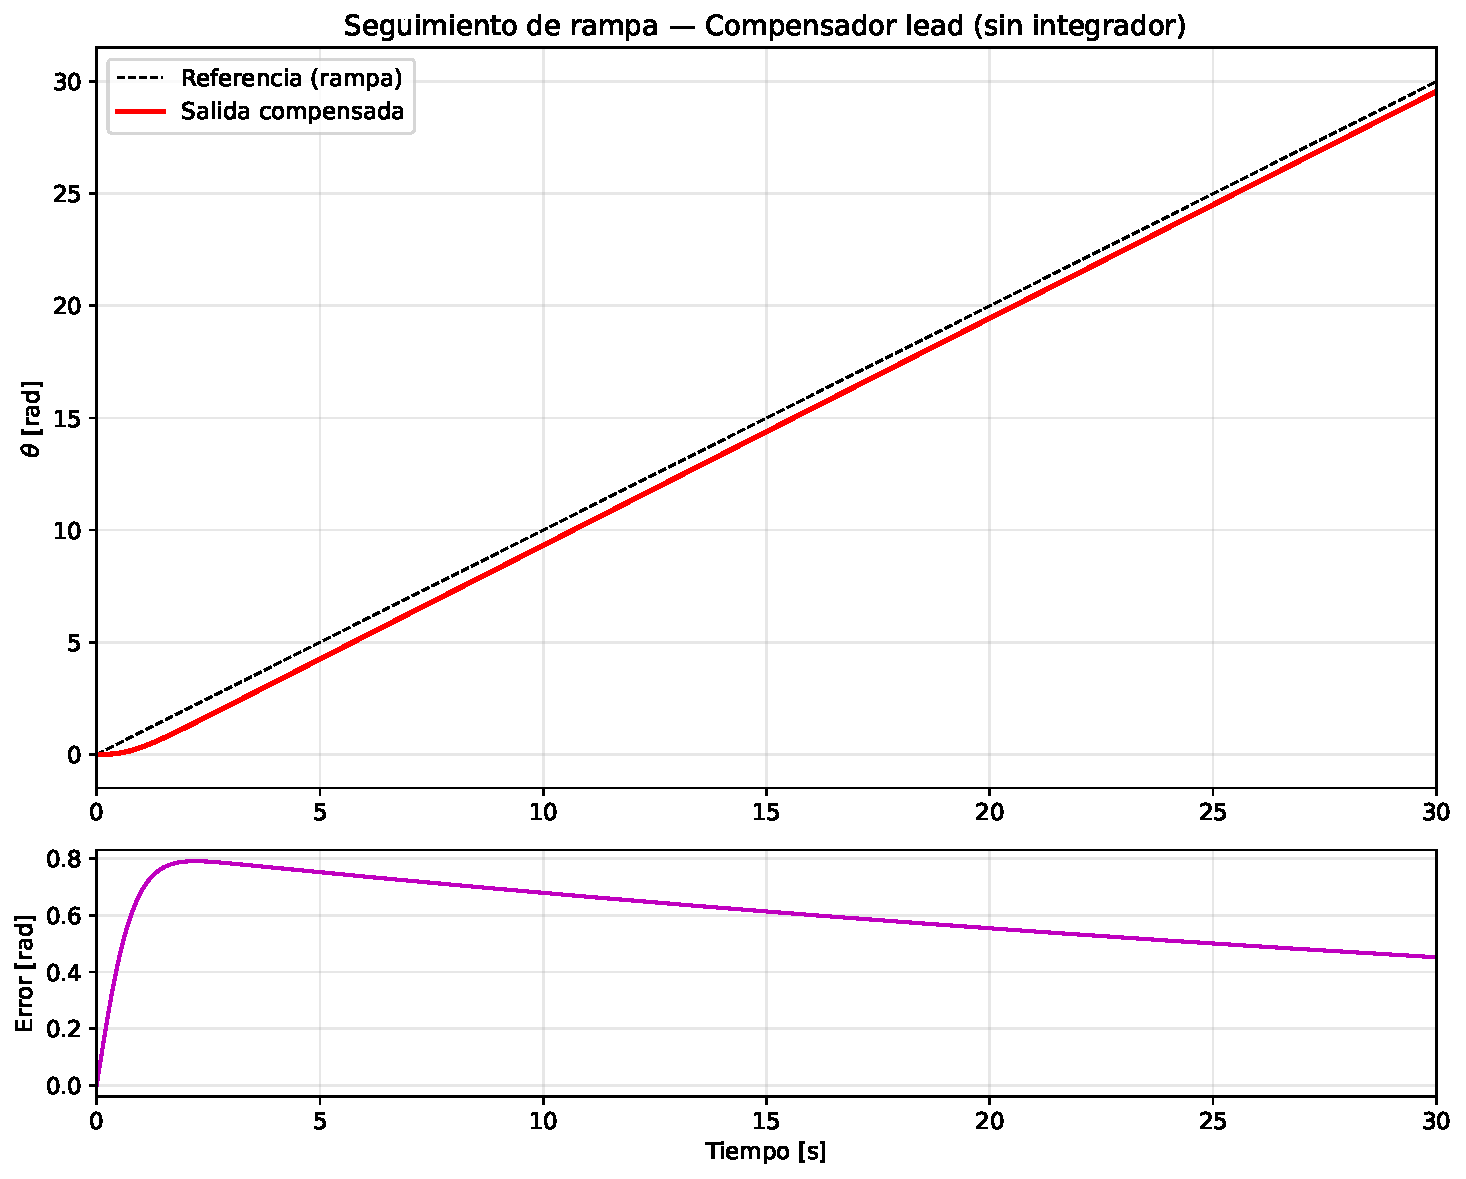
\includegraphics[width=0.85\textwidth]{rampa_lead.pdf}
\caption{Seguimiento de rampa con compensador lead (sin integrador). Se observa un error constante en régimen permanente.}
\label{fig:rampa_lead}
\end{figure}

El sistema compensado sigue siendo Tipo~1, por lo que el error ante rampa es constante y finito ($e_{ss} = 1/K_v$). El compensador lead mejoró el transitorio pero \textbf{no resolvió} el seguimiento de rampa. Numéricamente:
%
\begin{equation}
    K_v = \lim_{s\to 0} s \cdot C(s) G(s) = 1{,}2281 \;\text{rad/s} \quad \Rightarrow \quad e_{ss} = \frac{1}{K_v} \approx 0{,}814 \;\text{rad}
\end{equation}

\subsubsection{B.e) Modificación del controlador para seguimiento de rampa}

Para lograr error nulo ante rampa, se agrega un integrador al controlador:
%
\begin{equation}
    C_{nuevo}(s) = C_{lead}(s) \cdot \frac{1}{s}
\end{equation}

Esto convierte el sistema a \textbf{Tipo 2} ($K_v = \infty$). El riesgo es que el integrador introduce $-90°$ de fase adicional, reduciendo el margen de fase. Se rediseñó el compensador lead con cero en $z_c = -0{,}5$ (más cercano al origen que el lead original con $z_c=-2$), obteniendo:
%
\begin{equation}
    C_{nuevo}(s) = 3{,}9375 \cdot \frac{s + 0{,}5}{s(s + 4{,}6845)}
\end{equation}
%
con margen de fase $\text{PM} = 36{,}25°$ (positivo, sistema estable).

\begin{figure}[H]
\centering
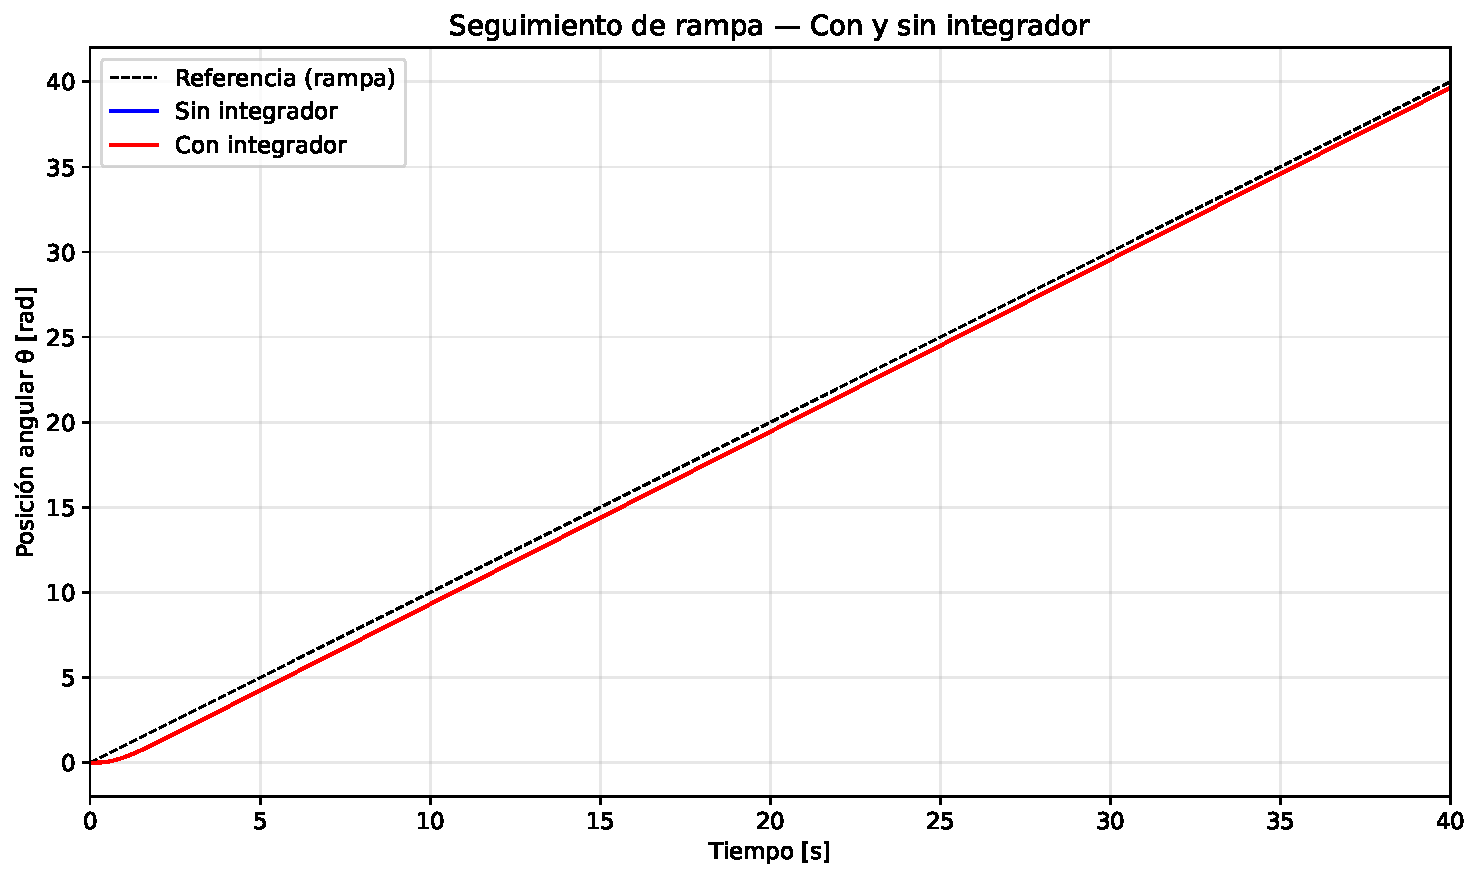
\includegraphics[width=0.85\textwidth]{rampa_con_integrador.pdf}
\caption{Seguimiento de rampa: comparación con y sin integrador.}
\label{fig:rampa_int}
\end{figure}

\begin{table}[H]
\centering
\caption{Verificación de especificaciones con $C_{nuevo}(s)$ (lead + integrador).}
\begin{tabular}{@{}lccl@{}}
\toprule
\textbf{Requisito} & \textbf{Obtenido} & \textbf{Límite} & \textbf{Cumple} \\
\midrule
$t_s$  & 7,16~s   & $\leq 7{,}5$~s & \checkmark \\
$M_p$  & 45,2\,\% & $\leq 15\,\%$  & $\times$ \\
$e_{rampa}$ & 0 & $0$ & \checkmark \\
\bottomrule
\end{tabular}
\end{table}

\paragraph{Observación.} El integrador satisface el seguimiento de rampa pero incrementa el sobrepico a 45\,\%, violando la especificación $M_p \leq 15\,\%$. Esto ilustra el compromiso fundamental: mayor tipo del sistema $\Rightarrow$ menor amortiguamiento. Para cumplir simultáneamente con todas las especificaciones se requeriría un controlador más sofisticado (PID, lead-lag con integrador, o diseño robusto).

\paragraph{Justificación.} El integrador adicional es necesario porque el sistema Tipo~1 tiene una limitación fundamental: no puede seguir referencias de tipo rampa con error nulo. Al pasar a Tipo~2, se logra $K_v = \infty$ y el error de velocidad desaparece. El compromiso es un margen de fase menor y mayor sobrepico.


% ============================================================================
% EJERCICIO 2
% ============================================================================
\newpage
\section{Ejercicio 2: Análisis y Control frente a Perturbaciones}

En este ejercicio se analiza la robustez del sistema de control ante la degradación del parámetro de fricción viscosa $B$, utilizando el modelo simplificado (se desprecia la dinámica eléctrica):
%
\begin{equation}
    G(s) = \frac{K}{s(Js+B)} = \frac{1}{s(s+B)}, \quad K = 1, \quad J = 1
    \label{eq:G2}
\end{equation}

El parámetro $B$ puede degradarse de $B = 0{,}5$ (nominal) a $B = -0{,}1$ (falla por fatiga térmica). Con $B < 0$, el polo $s = -B = 0{,}1$ se encuentra en el semiplano derecho.

% =========================================================================
\subsection{Parte A — Análisis de Sensibilidad y Robustez}
% =========================================================================

\subsubsection{A.a) Diagrama de Nyquist — Sistema nominal}

La Figura~\ref{fig:ej2_nyquist_nom} muestra el diagrama de Nyquist de $G(s)$ con $B = 0{,}5$.

\begin{figure}[H]
\centering
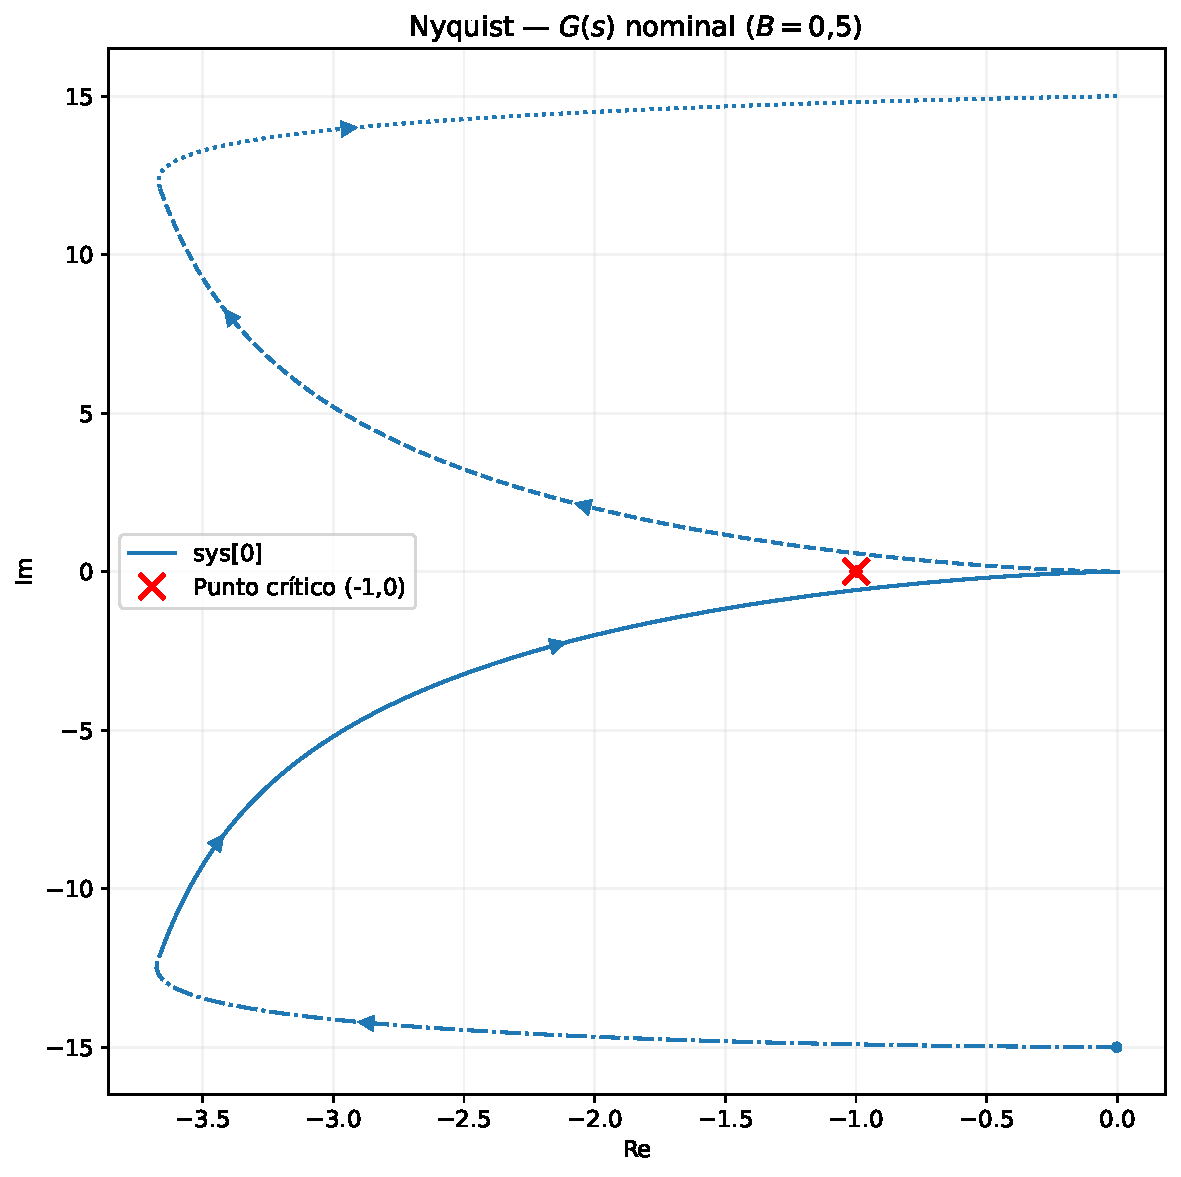
\includegraphics[width=0.7\textwidth]{ej2_nyquist_nominal.pdf}
\caption{Diagrama de Nyquist del sistema nominal ($B = 0{,}5$).}
\label{fig:ej2_nyquist_nom}
\end{figure}

Aplicando el criterio de Nyquist ($Z = N + P$):
\begin{itemize}
    \item $P = 0$ (no hay polos de $G(s)$ en el SPD; los polos son $s = 0$ y $s = -0{,}5$).
    \item $N = 0$ (la curva no rodea el punto $(-1, 0)$).
    \item $Z = 0 + 0 = 0$ $\Rightarrow$ \textbf{el sistema es estable en lazo cerrado}.
\end{itemize}

\subsubsection{A.b) Simulación de falla}

Se simula el sistema en lazo cerrado ($C(s) = 1$) ante escalón unitario, con $B$ cambiando de 0,5 a $-0{,}1$ en $t = 15$~s. Al ser un sistema \textbf{LTV} (variante en el tiempo), se usa espacio de estados con integración numérica:
%
\begin{equation}
    \dot{\theta} = \omega, \quad \dot{\omega} = -\frac{B(t)}{J}\omega + \frac{K}{J}(r - \theta)
\end{equation}

\begin{figure}[H]
\centering
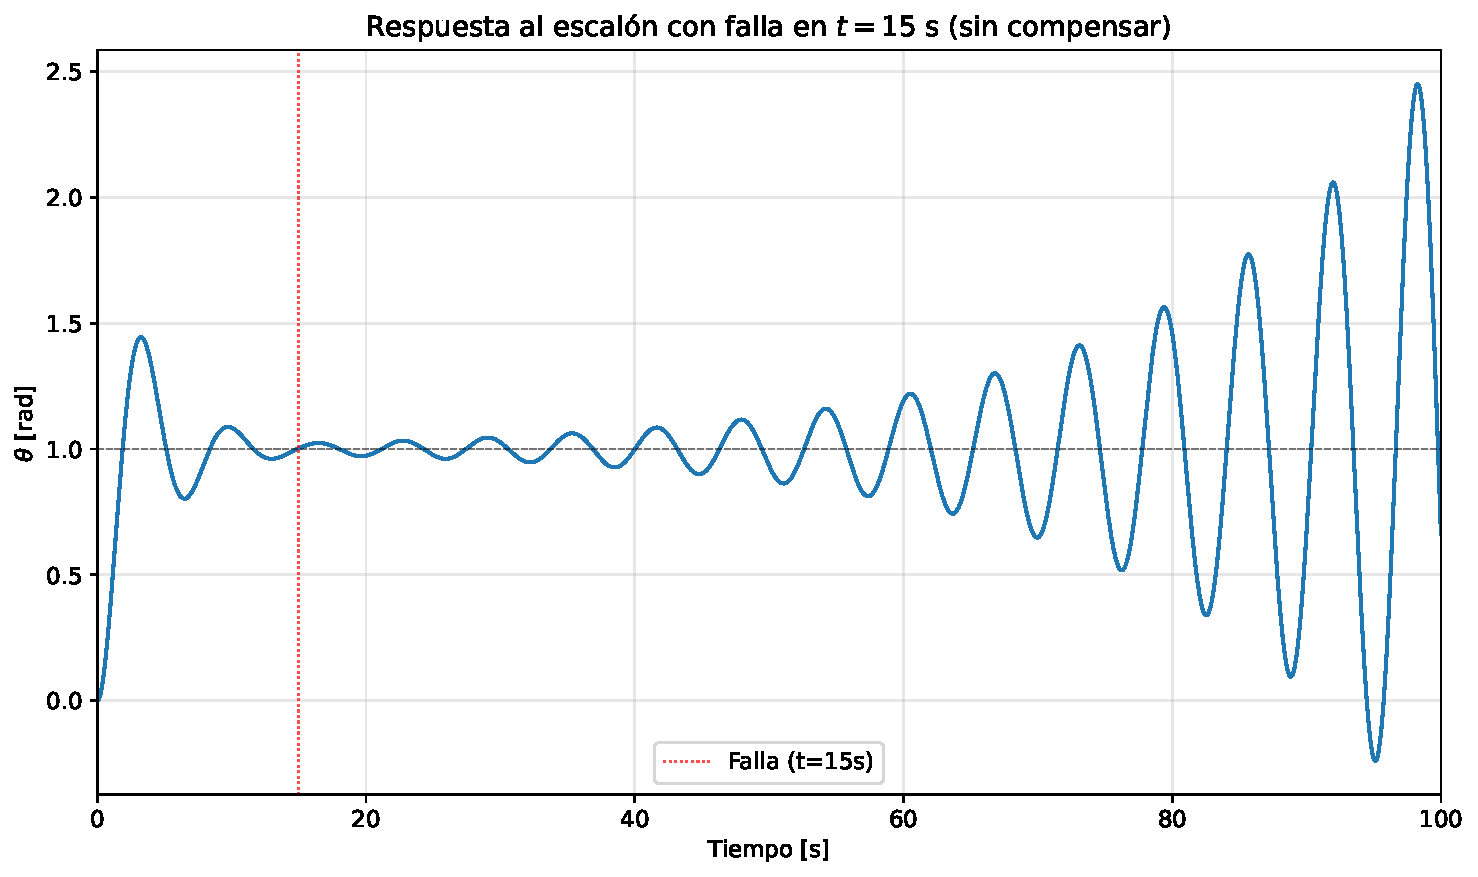
\includegraphics[width=0.85\textwidth]{ej2_falla_sin_comp.pdf}
\caption{Respuesta al escalón con falla en $t = 15$~s (sin compensar). La salida diverge.}
\label{fig:ej2_falla}
\end{figure}

El sistema \textbf{se vuelve inestable} tras la falla: con $B = -0{,}1$, la planta tiene un polo en $s = +0{,}1$ y la realimentación unitaria no alcanza para estabilizar.

\subsubsection{A.c) Root Locus comparativo}

\begin{figure}[H]
\centering
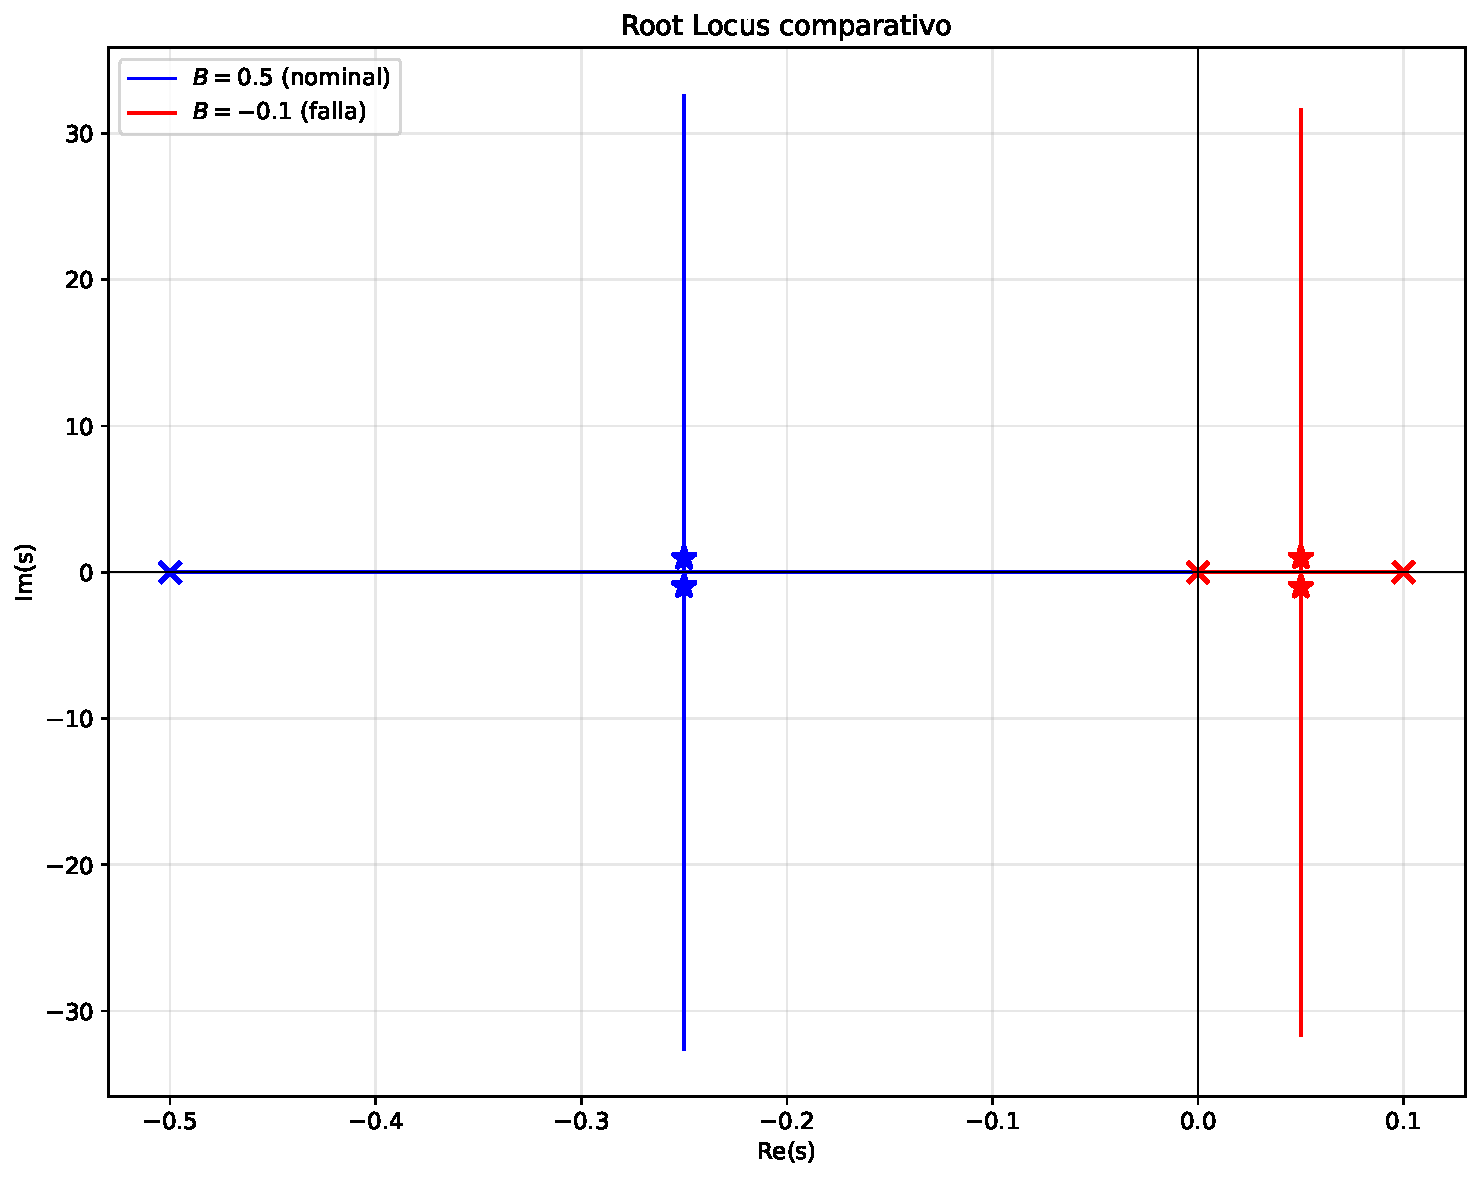
\includegraphics[width=0.85\textwidth]{ej2_rlocus_comparativo.pdf}
\caption{Root Locus: nominal ($B = 0{,}5$, azul) vs falla ($B = -0{,}1$, rojo). Las estrellas marcan polos de LC con $K = 1$.}
\label{fig:ej2_rlocus}
\end{figure}

\begin{itemize}
    \item \textbf{Nominal}: polos de LA en $s = 0$ y $s = -0{,}5$. El root locus parte hacia la izquierda $\Rightarrow$ estable para $K > 0$.
    \item \textbf{Falla}: polos de LA en $s = 0$ y $s = +0{,}1$. Una rama del RL parte del SPD. Con $K = 1$, al menos un polo de LC tiene $\text{Re}(s) > 0$ $\Rightarrow$ inestable.
\end{itemize}

\subsubsection{A.d) Propuesta de compensador}

Se propone un \textbf{compensador lead (adelanto de fase)}:
\begin{itemize}
    \item Aporta fase positiva $\Rightarrow$ incrementa el margen de fase.
    \item Mayor PM $\Rightarrow$ mayor tolerancia a la degradación de $B$.
    \item En el Nyquist, el lead ``aleja'' la curva del punto $(-1, 0)$.
    \item Un \textbf{lag} empeoraría el transitorio (reduce ancho de banda).
    \item Un \textbf{lead-lag} sería innecesariamente complejo para este caso.
\end{itemize}

Se normaliza la ganancia DC a 1 ($C(0) = K_c \cdot z/p = 1 \Rightarrow K_c = p/z$) para no alterar el error de posición. Esto es posible porque $z/p < 1$ en un lead, y $K_c$ compensa exactamente.

% =========================================================================
\subsection{Parte B — Diseño de Compensador para Estabilidad Robusta}
% =========================================================================

\subsubsection{B.a) Diseño para MF = 35$^{\circ}$, 50$^{\circ}$, 65$^{\circ}$}

El procedimiento de diseño por respuesta en frecuencia es:
\begin{enumerate}
    \item Fase adicional necesaria: $\phi_{max} = \text{PM}_{deseado} - \text{PM}_{actual} + 5°$ (margen de seguridad).
    \item Parámetro del lead: $\alpha = \frac{1 - \sin\phi_{max}}{1 + \sin\phi_{max}}$.
    \item Frecuencia de máxima fase: $\omega_m$ donde $|G(j\omega_m)| = \sqrt{\alpha}$.
    \item Cero $z = \omega_m\sqrt{\alpha}$, polo $p = \omega_m/\sqrt{\alpha}$, ganancia $K_c = p/z$.
\end{enumerate}

\begin{table}[H]
\centering
\caption{Parámetros de los tres compensadores lead diseñados ($B = 0{,}5$, PM sin compensar = 28°).}
\label{tab:ej2_leads}
\begin{tabular}{@{}cccccc@{}}
\toprule
\textbf{PM objetivo} & \textbf{PM obtenido} & $\alpha$ & $z$ & $p$ & $K_c$ \\
\midrule
35$^{\circ}$ & 37,3$^{\circ}$ & 0,656 & 0,856 & 1,304 & 1,524 \\
50$^{\circ}$ & 49,1$^{\circ}$ & 0,376 & 0,754 & 2,006 & 2,661 \\
65$^{\circ}$ & 60,9$^{\circ}$ & 0,198 & 0,649 & 3,271 & 5,040 \\
\bottomrule
\end{tabular}
\end{table}

En todos los casos $C(0) = K_c \cdot z/p = 1{,}00$, verificando la normalización de ganancia DC.

\subsubsection{B.b) Verificación por Bode}

\begin{figure}[H]
\centering
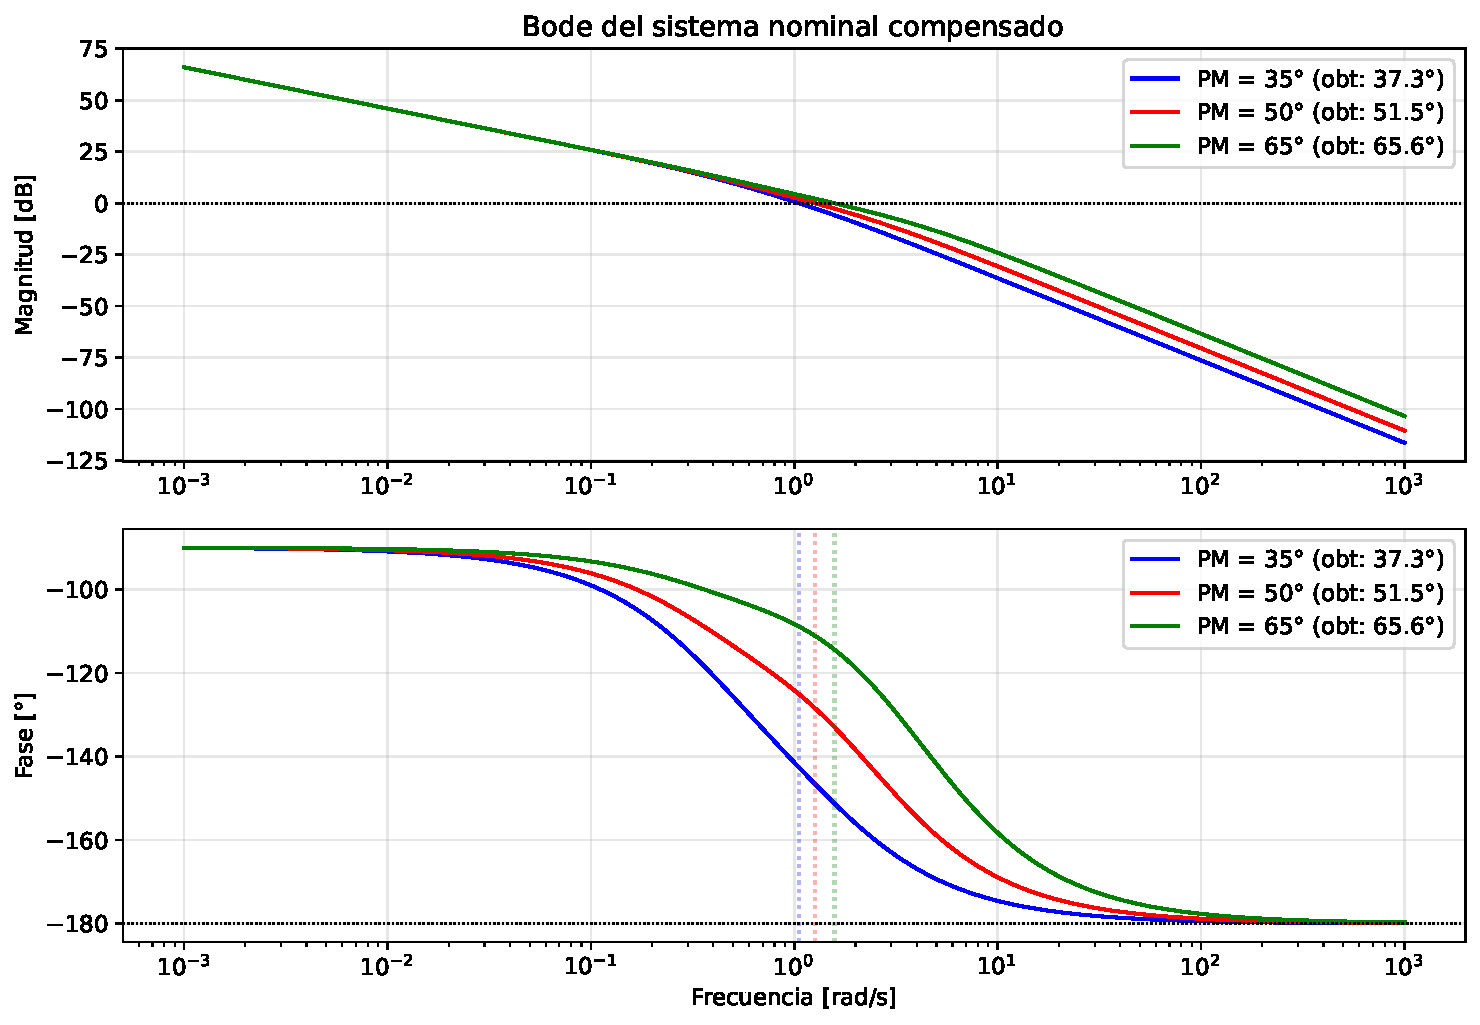
\includegraphics[width=0.85\textwidth]{ej2_bode_3compensadores.pdf}
\caption{Diagrama de Bode del sistema nominal compensado para los tres valores de PM.}
\label{fig:ej2_bode}
\end{figure}

Se verifica que los márgenes de fase obtenidos coinciden con los objetivos. La ganancia en baja frecuencia es idéntica para los tres casos (normalización DC). En este diseño normalizado, $\omega_{cp}$ \emph{aumenta} con el PM: un objetivo de fase mayor requiere un $\alpha$ menor, lo que desplaza la frecuencia de máxima fase $\omega_m$ hacia valores más altos, elevando la frecuencia de cruce.

\begin{table}[H]
\centering
\caption{Métricas de desempeño del sistema nominal compensado (lazo cerrado, escalón unitario).}
\begin{tabular}{@{}cccccc@{}}
\toprule
\textbf{PM obj.} & \textbf{PM obt.} & $\omega_{cp}$ [rad/s] & $M_p$ [\%] & $t_s$ [s] & \textbf{Polo lead $p$} \\
\midrule
35° & 37,3° & 1,056 & 33,4 & 9,3 & 1,304 \\
50° & 49,1° & 1,229 & 20,8 & 5,1 & 2,005 \\
65° & 60,9° & 1,457 &  9,5 & 3,5 & 3,271 \\
\bottomrule
\end{tabular}
\end{table}

\subsubsection{B.c) Respuesta al escalón con falla}

\begin{figure}[H]
\centering
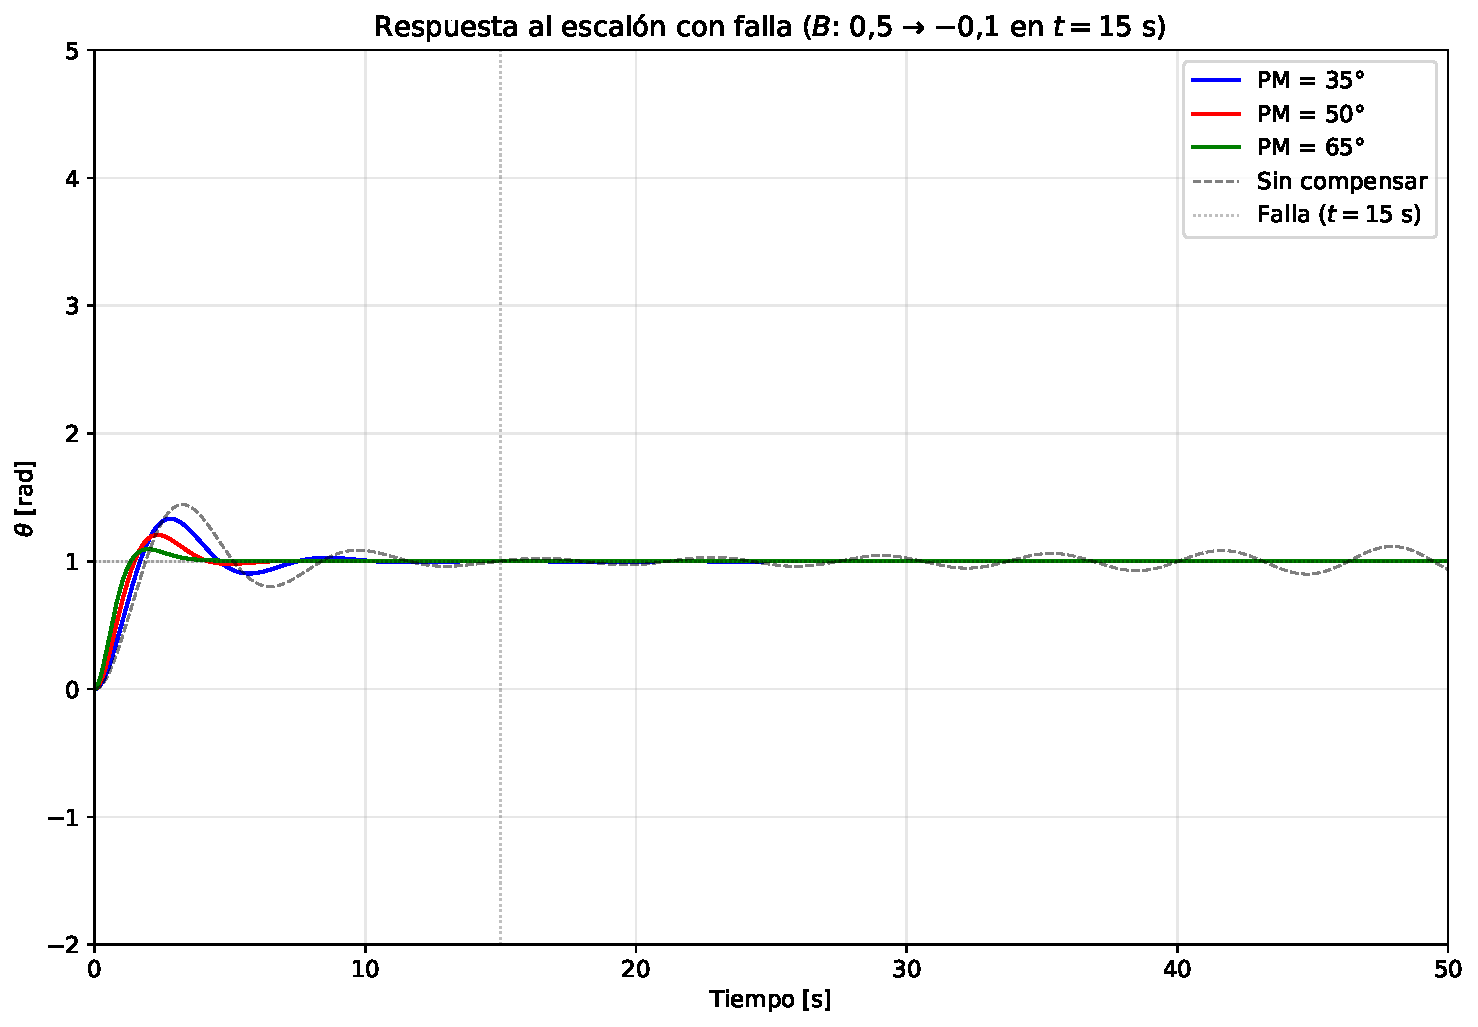
\includegraphics[width=0.85\textwidth]{ej2_falla_3compensadores.pdf}
\caption{Respuesta al escalón con falla ($B$: 0,5 $\to$ $-0{,}1$ en $t = 15$~s) para los tres compensadores. Sin compensar (línea punteada) diverge.}
\label{fig:ej2_falla3}
\end{figure}

\begin{itemize}
    \item A mayor margen de fase, la recuperación post-falla es más suave y amortiguada.
    \item El sistema \textbf{se parece cada vez más a uno de primer orden} al incrementar el PM: el sobrepico desaparece y la respuesta es monótona. Esto se debe a que el mayor amortiguamiento aleja los polos de LC del eje imaginario.
    \item El tiempo de establecimiento post-falla es \emph{menor} con PM = 65° que con PM = 35° (mayor ancho de banda), pero el sistema es más amortiguado y la estabilidad frente a degradación paramétrica está mejor garantizada.
\end{itemize}

\subsubsection{B.d) Análisis de Nyquist y desventajas}

\begin{figure}[H]
\centering
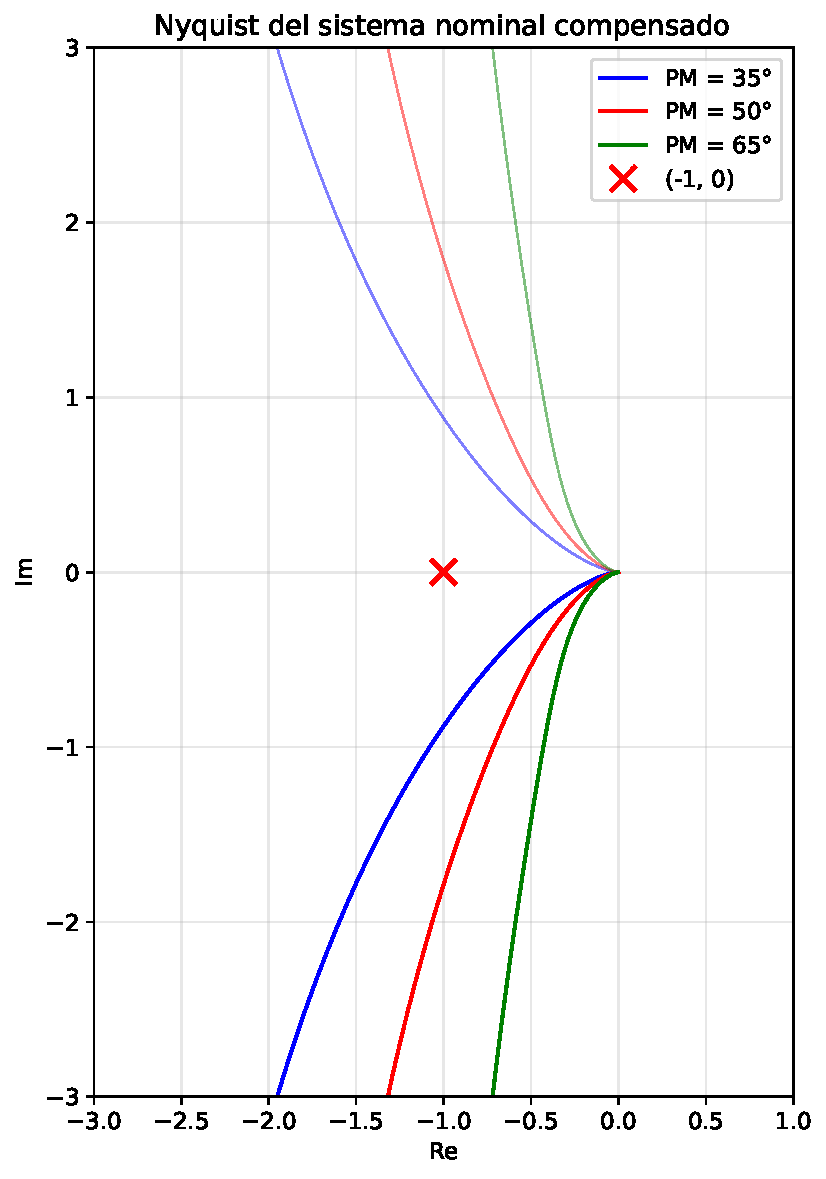
\includegraphics[width=0.7\textwidth]{ej2_nyquist_compensado.pdf}
\caption{Nyquist del sistema nominal compensado. El compensador ``aleja'' la curva del punto $(-1, 0)$.}
\label{fig:ej2_nyquist_comp}
\end{figure}

\paragraph{¿Cómo ``aleja'' el compensador la curva de $(-1,0)$?} El lead aporta fase positiva en la frecuencia de cruce, lo que \textbf{rota} la curva de Nyquist en sentido antihorario cerca del punto crítico. A mayor PM, mayor es la distancia mínima entre la curva y $(-1, 0)$, otorgando mayor robustez frente a la degradación de $B$.

\paragraph{Desventajas de incrementar el MF:}
\begin{enumerate}
    \item \textbf{Polo del compensador más alejado} ($p$ crece) $\Rightarrow$ mayor amplificación de ruido en alta frecuencia y esfuerzo de control más agresivo.
    \item \textbf{Mayor sobrepico inicial} al aumentar $\omega_{cp}$, antes de que el mayor amortiguamiento lo reduzca: el compromiso es no-lineal.
    \item \textbf{Mayor sensibilidad al ruido de medición}: el polo alejado amplifica frecuencias altas.
    \item \textbf{Incremento de $K_c$}: la ganancia del compensador crece con $1/\alpha$, lo que puede saturar el actuador.
\end{enumerate}

Existe un \textbf{compromiso} entre robustez (MF alto) y desempeño dinámico (MF moderado). El valor adecuado depende del rango de variación esperado de los parámetros de la planta.


% ============================================================================
% CONCLUSIONES
% ============================================================================
\newpage
\section{Conclusiones}

En este trabajo se diseñaron controladores para un sistema de orientación de rotor VTOL accionado por motor DC, abordando dos escenarios complementarios.

\textbf{Ejercicio 1}: se partió de un modelo completo del motor DC (3er orden, Tipo~1) y se diseñó un compensador lead por root locus que satisface las especificaciones de transitorio ($t_s = 4{,}84$~s, $M_p = 11{,}65\,\%$), pero que no puede cumplir simultáneamente la especificación de rechazo de perturbación ($e_{pert} = 65\,\% \gg 5\,\%$): al conservar la ganancia DC del lazo ($C(0)\approx 1$), el error ante torque de carga permanece elevado. Para lograr seguimiento de rampa con error nulo se añadió un integrador (Tipo~2), pero esto elevó el sobrepico a $45\,\%$, superando el límite del $15\,\%$. Esto evidencia que las tres especificaciones simultáneas no pueden satisfacerse con un lead simple ni con lead más integrador; se requeriría un controlador más sofisticado (PID, lead-lag con integrador).

\textbf{Ejercicio 2}: con un modelo simplificado, se analizó la vulnerabilidad del sistema ante degradación del parámetro de fricción $B$. Se demostró que sin compensador, un cambio de $B = 0{,}5$ a $B = -0{,}1$ destruye la estabilidad. Se diseñaron tres compensadores lead normalizados (PM = 35°, 50° y 65°) y se verificó que mayores márgenes de fase otorgan mayor robustez y mayor amortiguamiento ante la falla, con la contrapartida de un polo del compensador más alejado en el eje real, mayor sensibilidad al ruido y mayor ganancia $K_c$.

\textbf{Lecciones clave}:
\begin{itemize}
    \item Los márgenes de estabilidad no son solo indicadores teóricos: determinan la tolerancia del sistema a variaciones paramétricas reales.
    \item El diseño por root locus y por respuesta en frecuencia (Bode) son complementarios: el primero permite ubicar polos de LC, el segundo da una medida directa de robustez.
    \item No existe un controlador ``óptimo'' universal: siempre hay un compromiso entre desempeño transitorio, precisión en régimen permanente y robustez frente a incertidumbres.
\end{itemize}

% ============================================================================
\end{document}
